% Options for packages loaded elsewhere
\PassOptionsToPackage{unicode}{hyperref}
\PassOptionsToPackage{hyphens}{url}
\documentclass[
]{article}
\usepackage{xcolor}
\usepackage[margin=1in]{geometry}
\usepackage{amsmath,amssymb}
\setcounter{secnumdepth}{5}
\usepackage{iftex}
\ifPDFTeX
  \usepackage[T1]{fontenc}
  \usepackage[utf8]{inputenc}
  \usepackage{textcomp} % provide euro and other symbols
\else % if luatex or xetex
  \usepackage{unicode-math} % this also loads fontspec
  \defaultfontfeatures{Scale=MatchLowercase}
  \defaultfontfeatures[\rmfamily]{Ligatures=TeX,Scale=1}
\fi
\usepackage{lmodern}
\ifPDFTeX\else
  % xetex/luatex font selection
\fi
% Use upquote if available, for straight quotes in verbatim environments
\IfFileExists{upquote.sty}{\usepackage{upquote}}{}
\IfFileExists{microtype.sty}{% use microtype if available
  \usepackage[]{microtype}
  \UseMicrotypeSet[protrusion]{basicmath} % disable protrusion for tt fonts
}{}
\makeatletter
\@ifundefined{KOMAClassName}{% if non-KOMA class
  \IfFileExists{parskip.sty}{%
    \usepackage{parskip}
  }{% else
    \setlength{\parindent}{0pt}
    \setlength{\parskip}{6pt plus 2pt minus 1pt}}
}{% if KOMA class
  \KOMAoptions{parskip=half}}
\makeatother
\usepackage{color}
\usepackage{fancyvrb}
\newcommand{\VerbBar}{|}
\newcommand{\VERB}{\Verb[commandchars=\\\{\}]}
\DefineVerbatimEnvironment{Highlighting}{Verbatim}{commandchars=\\\{\}}
% Add ',fontsize=\small' for more characters per line
\usepackage{framed}
\definecolor{shadecolor}{RGB}{248,248,248}
\newenvironment{Shaded}{\begin{snugshade}}{\end{snugshade}}
\newcommand{\AlertTok}[1]{\textcolor[rgb]{0.94,0.16,0.16}{#1}}
\newcommand{\AnnotationTok}[1]{\textcolor[rgb]{0.56,0.35,0.01}{\textbf{\textit{#1}}}}
\newcommand{\AttributeTok}[1]{\textcolor[rgb]{0.13,0.29,0.53}{#1}}
\newcommand{\BaseNTok}[1]{\textcolor[rgb]{0.00,0.00,0.81}{#1}}
\newcommand{\BuiltInTok}[1]{#1}
\newcommand{\CharTok}[1]{\textcolor[rgb]{0.31,0.60,0.02}{#1}}
\newcommand{\CommentTok}[1]{\textcolor[rgb]{0.56,0.35,0.01}{\textit{#1}}}
\newcommand{\CommentVarTok}[1]{\textcolor[rgb]{0.56,0.35,0.01}{\textbf{\textit{#1}}}}
\newcommand{\ConstantTok}[1]{\textcolor[rgb]{0.56,0.35,0.01}{#1}}
\newcommand{\ControlFlowTok}[1]{\textcolor[rgb]{0.13,0.29,0.53}{\textbf{#1}}}
\newcommand{\DataTypeTok}[1]{\textcolor[rgb]{0.13,0.29,0.53}{#1}}
\newcommand{\DecValTok}[1]{\textcolor[rgb]{0.00,0.00,0.81}{#1}}
\newcommand{\DocumentationTok}[1]{\textcolor[rgb]{0.56,0.35,0.01}{\textbf{\textit{#1}}}}
\newcommand{\ErrorTok}[1]{\textcolor[rgb]{0.64,0.00,0.00}{\textbf{#1}}}
\newcommand{\ExtensionTok}[1]{#1}
\newcommand{\FloatTok}[1]{\textcolor[rgb]{0.00,0.00,0.81}{#1}}
\newcommand{\FunctionTok}[1]{\textcolor[rgb]{0.13,0.29,0.53}{\textbf{#1}}}
\newcommand{\ImportTok}[1]{#1}
\newcommand{\InformationTok}[1]{\textcolor[rgb]{0.56,0.35,0.01}{\textbf{\textit{#1}}}}
\newcommand{\KeywordTok}[1]{\textcolor[rgb]{0.13,0.29,0.53}{\textbf{#1}}}
\newcommand{\NormalTok}[1]{#1}
\newcommand{\OperatorTok}[1]{\textcolor[rgb]{0.81,0.36,0.00}{\textbf{#1}}}
\newcommand{\OtherTok}[1]{\textcolor[rgb]{0.56,0.35,0.01}{#1}}
\newcommand{\PreprocessorTok}[1]{\textcolor[rgb]{0.56,0.35,0.01}{\textit{#1}}}
\newcommand{\RegionMarkerTok}[1]{#1}
\newcommand{\SpecialCharTok}[1]{\textcolor[rgb]{0.81,0.36,0.00}{\textbf{#1}}}
\newcommand{\SpecialStringTok}[1]{\textcolor[rgb]{0.31,0.60,0.02}{#1}}
\newcommand{\StringTok}[1]{\textcolor[rgb]{0.31,0.60,0.02}{#1}}
\newcommand{\VariableTok}[1]{\textcolor[rgb]{0.00,0.00,0.00}{#1}}
\newcommand{\VerbatimStringTok}[1]{\textcolor[rgb]{0.31,0.60,0.02}{#1}}
\newcommand{\WarningTok}[1]{\textcolor[rgb]{0.56,0.35,0.01}{\textbf{\textit{#1}}}}
\usepackage{graphicx}
\makeatletter
\newsavebox\pandoc@box
\newcommand*\pandocbounded[1]{% scales image to fit in text height/width
  \sbox\pandoc@box{#1}%
  \Gscale@div\@tempa{\textheight}{\dimexpr\ht\pandoc@box+\dp\pandoc@box\relax}%
  \Gscale@div\@tempb{\linewidth}{\wd\pandoc@box}%
  \ifdim\@tempb\p@<\@tempa\p@\let\@tempa\@tempb\fi% select the smaller of both
  \ifdim\@tempa\p@<\p@\scalebox{\@tempa}{\usebox\pandoc@box}%
  \else\usebox{\pandoc@box}%
  \fi%
}
% Set default figure placement to htbp
\def\fps@figure{htbp}
\makeatother
\setlength{\emergencystretch}{3em} % prevent overfull lines
\providecommand{\tightlist}{%
  \setlength{\itemsep}{0pt}\setlength{\parskip}{0pt}}
\usepackage{bookmark}
\IfFileExists{xurl.sty}{\usepackage{xurl}}{} % add URL line breaks if available
\urlstyle{same}
\hypersetup{
  pdftitle={Trabajo final},
  pdfauthor={Lucio Enrique Cornejo Ramírez},
  hidelinks,
  pdfcreator={LaTeX via pandoc}}

\title{Trabajo final}
\author{Lucio Enrique Cornejo Ramírez}
\date{2025-06-16}

\begin{document}
\maketitle

{
\setcounter{tocdepth}{3}
\tableofcontents
}
\subsection{Introducción}\label{introducciuxf3n}

\subsubsection{Marco del problema}\label{marco-del-problema}

Entre los costos que más desastibilizan económicamente a las personas,
se encuentra el pago por procedimientos médicos. Estos precios pueden
variar en gran medida dependiendo de características del paciente, como
detallaremos más adelante.

En ese sentido, resulta de gran valor predecir adecuadamente el costo
que un seguro médico cubrirá, respecto a un procedimiento médico. Para
un paciente, aquella predicción puede servir para que planifique qué
tanto sería desestabilizado económicamente debido a algún tipo de
procedimiento particular. Por otro lado, también para las aseguradoras
resulta útil aquellas predicciones, ya que pueden anticipar qué tanto
dinero estarían perdiendo por el monto a cubrir de la operación; además,
con ese conocimiento pueden monitorear mejor qué pedidos de cobertura
resultan anómalos, potencialmente fraudulentos.

\subsubsection{Plan de modelamiento}\label{plan-de-modelamiento}

Anteriormente, hemos planteado como variable por predecir a la cantidad
monetaria que la aseguradora de un paciente cubrirá debido a un
procedimiento médico. Note que aquel monto está muy relacionado al
precio que paga el paciente luego que el seguro descuenta parte del
costo del procedimiento médico \ldots{} ese monto, que denominaremos
\texttt{charges}, se intentará predecir.

Asimismo, vale recalcar la influencia de los gastos del hospital debido
al procedimiento médico, variable que denotaremos
\texttt{Hospital\_expenditure}, sobre \texttt{charges}.

Para el modelamiento, se considerará además las siguientes
características del paciente:

\begin{itemize}
\tightlist
\item
  Sexo (\texttt{age})
\item
  Si fuma o no (\texttt{smoker})
\item
  Región de la que provee (\texttt{region})
\item
  Edad (\texttt{age})
\item
  Índice de masa corporal (\texttt{bmi})
\item
  Cantidad de hijos e hijas (\texttt{children})
\item
  Costo médico que pagaría en caso no se aplicase seguro médico
  (\texttt{Claim\_Amount})
\item
  Número de procedimientos pasados (\texttt{past\_consultations})
\item
  Número de pasos que realizó en cierto día (\texttt{num\_of\_steps})
\item
  Número de veces que ha sido hospitalizado
  (\texttt{Number\_of\_past\_hospitalizations})
\item
  Salario anual (\texttt{Anual\_Salary})
\end{itemize}

\subsection{Materiales y métodos}\label{materiales-y-muxe9todos}

\subsubsection{Datos/Observaciones}\label{datosobservaciones}

Las observaciones que consideraremos para este proyecto fueron
descargadas de este sitio
\href{https://www.kaggle.com/datasets/shubhamsingh57/ml-model-practice-linear-regression/data}{web}.

Estos datos son de distintos pacientes que recibieron algún tipo de
tratamiento médico, de los cuales se tienen variables recopiladas, como
edad, sexo, si fuma o no, etc. Así, descartamos que los datos consistan
de una serie de tiempo.

No obstante, aquella página web no provee información más específica
sobre el origen de los datos. Por ejemplo, si han sido recopilados en un
único hospital, o en diversos hospitales, pero de qué país, etc.

Aún así, en esta investigación, no solo se considera la predicción de la
variable mencionada, sino también cómo es que influyen las variables que
emplearemos como regresores, en la predicción final. Por ejemplo, si su
relación es directa o inversamente proporcional.

A continuación justificamos el posible uso de los caracteres presentes
en los datos, como covariables:

\begin{itemize}
\tightlist
\item
  \textbf{Sexo}: Debido al riesgo y costos distintos entre hombres y
  mujeres, para ciertos tipos de operaciones; por ejemplo, parto.
\item
  \textbf{Si fuma o no}: Pues fumar aumenta la probabilidad de
  desarrollar complicaciones médicas
\item
  \textbf{Región de la que provee}: Ya que el costo de un procedimiento
  médico puede variar mucho por región, así que también varía cuánto
  cubriría una aseguradora.
\item
  \textbf{Edad}: Puesto que pacientes mayores suelen requerir más
  cuidados.
\item
  \textbf{Índice de masa corporal}: En base a que un IMC elevado está
  asociado a mayores riesgos durante cirugías.
\item
  \textbf{Cantidad de hijos e hijas}: Esto puede influir en el tipo de
  cobertura familiar (de seguro) que tiene el paciente.
\item
  \textbf{Costo médico que pagaría en caso no se aplicase seguro
  médico}: Importante incluirlo, pues incluso se espera que presente una
  fuerte correlación positiva con la variable por predecir.
\item
  \textbf{Número de procedimientos pasados}: Puede resultar útil en base
  a que pacientes con muchos procedimientos suelen tener enfermedades
  crónicas, por lo que se esperaría una mayor cobertura.
\item
  \textbf{Número de pasos que realizó en cierto día}: Esta variable
  tampoco se explica en la fuente, pero la podemos considerar como una
  medida de la condición física de una persona, qué tan activa es.
\item
  \textbf{Número de veces que ha sido hospitalizado}: Pues más
  hospitalizaciones implican mayor riesgo en la operación, aumentando
  posiblemente así los costos que cubre la aseguradora.
\item
  \textbf{Salario anual}: Como indicador de nivel socioeconómico, se
  espera que pacientes con ingresos altos cuenten con aseguradoras que
  cubren mayor parte el costo por intervención médica.
\end{itemize}

\subsubsection{Itinerario metodológico de la
modelización}\label{itinerario-metodoluxf3gico-de-la-modelizaciuxf3n}

A continuación, describrimos los pasos a seguir para la construcción de
diferentes modelos de predicción:

\begin{enumerate}
\def\labelenumi{\arabic{enumi}.}
\item
  Descarte de observaciones que presenten algún valor faltante para
  cualquier variable.
\item
  Gráficos de dispersión para pares de variables
\item
  Debido al máximo establecido en este proyecto, respecto al número de
  covariables, calculamos las correlaciones múltiples
\item
  Filtro de observaciones al azar, debido a máximo establecido en este
  proyecto.
\item
  Limpieza de datos
\item
  Construcción del modelo OLS, empleando todas las covariables
\item
  Gráficos de valores observados y residuos contra valores estimados.
  Interpretar R\^{}2
\item
  Emplear el test de Levine y Shapiro para averiguar la homocedasticidad
  y la normalidad.
\item
  En caso positivo, evaluar por medio de ANOVA si el modelo tiene
  sentido. En caso positivo, determinar qué variables explicativas
  tienen sentido.
\item
  Si se encuentran puntos aberrantes, recorrer el modelo sin aquellos y
  repetir los pasos mencionados.
\item
  Emplear selección por delante, para atrás y stepwise.
\item
  Ejecutar los tests de tipo ANOVA
\item
  En caso el test ANOVA relevante resulte positivo, incluir los tests
  post-hoc.
\end{enumerate}

\subsection{Resultados}\label{resultados}

\subsubsection{Carga de datos}\label{carga-de-datos}

A continuación, mostramos los datos descargados del sitio web mencionado
en la sección previa.

\begin{Shaded}
\begin{Highlighting}[]
\FunctionTok{library}\NormalTok{(dplyr)}
\end{Highlighting}
\end{Shaded}

\begin{verbatim}
## 
## Attaching package: 'dplyr'
\end{verbatim}

\begin{verbatim}
## The following objects are masked from 'package:stats':
## 
##     filter, lag
\end{verbatim}

\begin{verbatim}
## The following objects are masked from 'package:base':
## 
##     intersect, setdiff, setequal, union
\end{verbatim}

\begin{Shaded}
\begin{Highlighting}[]
\FunctionTok{library}\NormalTok{(tidyr)}
\FunctionTok{library}\NormalTok{(ggplot2)}
\FunctionTok{library}\NormalTok{(reshape2)}
\end{Highlighting}
\end{Shaded}

\begin{verbatim}
## 
## Attaching package: 'reshape2'
\end{verbatim}

\begin{verbatim}
## The following object is masked from 'package:tidyr':
## 
##     smiths
\end{verbatim}

\begin{Shaded}
\begin{Highlighting}[]
\NormalTok{datos }\OtherTok{\textless{}{-}}\NormalTok{ readr}\SpecialCharTok{::}\FunctionTok{read\_csv}\NormalTok{(}\StringTok{"./new\_insurance\_data.csv"}\NormalTok{)}
\end{Highlighting}
\end{Shaded}

\begin{verbatim}
## Rows: 1338 Columns: 13
## -- Column specification ---------------------------------------------------------------------------------------------------------------------------------------------------------------------------------
## Delimiter: ","
## chr  (3): sex, smoker, region
## dbl (10): age, bmi, children, Claim_Amount, past_consultations, num_of_steps, Hospital_expenditure, Number_of_past_hospitalizations, Anual_Salary, charges
## 
## i Use `spec()` to retrieve the full column specification for this data.
## i Specify the column types or set `show_col_types = FALSE` to quiet this message.
\end{verbatim}

\begin{Shaded}
\begin{Highlighting}[]
\NormalTok{dplyr}\SpecialCharTok{::}\FunctionTok{glimpse}\NormalTok{(datos)}
\end{Highlighting}
\end{Shaded}

\begin{verbatim}
## Rows: 1,338
## Columns: 13
## $ age                             <dbl> 18, 18, 18, 18, 18, 18, 18, 18, 18, 18, 19, 19, 19, 19, 19, 19, NA, 19, 19, 20, 21, 21, 21, 21, 18, 18, 19, 18, 18, 19, 19, 19, 18, 18, 18, NA, 19, 18, 18, 18~
## $ sex                             <chr> "male", "male", "male", "male", "male", "male", "male", "male", "male", "male", "male", "male", "male", "male", "male", "male", "male", "male", "male", "male"~
## $ bmi                             <dbl> 23.210, 30.140, 33.330, 33.660, 34.100, 34.430, 37.290, 41.140, 43.010, 53.130, 19.800, 20.300, 20.700, 27.600, 28.700, NA, 34.100, 34.400, 35.400, 33.330, 23~
## $ children                        <dbl> 0, 0, 0, 0, 0, 0, 0, 0, 0, 0, 0, 0, 0, 0, 0, 0, 0, 0, 0, 0, 0, 0, 0, 0, 0, 0, 0, 0, 0, 0, 0, 0, 0, 0, 0, 0, 0, 0, 0, 0, 0, 0, 0, 0, 0, 0, 0, 0, 0, 0, 0, 0, 0,~
## $ smoker                          <chr> "no", "no", "no", "no", "no", "no", "no", "no", "no", "no", "no", "no", "no", "no", "no", "no", "no", "no", "no", "no", "no", "no", "no", "no", "no", "no", "n~
## $ Claim_Amount                    <dbl> 29087.543, 39053.674, 39023.628, 28185.393, 14697.859, 26488.339, 33217.365, 46770.585, 9715.650, 17046.585, 16980.214, 1920.136, 3927.892, 46780.546, 36778.5~
## $ past_consultations              <dbl> 17, 7, 19, 11, 16, 20, 13, 12, 17, 19, 2, NA, 4, 8, 3, 15, 3, 2, 2, 14, 10, 6, 15, 7, 19, 9, 6, 9, 3, 10, 5, 9, 13, 7, 2, 17, 5, 13, 16, 15, 14, 9, 21, 8, 8, ~
## $ num_of_steps                    <dbl> 715428, 699157, 702341, 700250, 711584, 717162, 699159, 706423, NA, 704425, 706796, 695430, 723928, 701227, 724149, 726642, 718891, 720340, 711546, 729642, 72~
## $ Hospital_expenditure            <dbl> 4720920.99, 4329831.68, 6884860.77, 4274773.55, 3787293.92, 3696160.70, 876529.19, 4486741.20, 9216440.48, 1458971.92, 4981702.85, 3786542.07, 5013944.64, NA,~
## $ Number_of_past_hospitalizations <dbl> 0, 0, 0, 0, 0, 0, 0, 0, 0, 0, 0, 0, NA, 0, 0, 0, 0, 0, 0, 0, 0, 0, 0, 0, 0, 0, 0, 0, 0, 0, 0, 0, 0, 0, 0, 0, 0, 0, 0, 0, 0, 0, 0, 0, 0, 0, 0, 0, 0, 0, 0, 0, 0~
## $ Anual_Salary                    <dbl> 55784970, 13700885, 73523107, 75819680, 23012320, NA, 69060666, 97193784, 58881972, 94261821, 70076110, 2747072, 94628895, 38421625, 17904619, 43544451, 23965~
## $ region                          <chr> "southeast", "southeast", "southeast", "southeast", "southeast", "southeast", "southeast", "southeast", "southeast", "southeast", "southwest", "southwest", "s~
## $ charges                         <dbl> 1121.874, 1131.507, 1135.941, 1136.399, 1137.011, 1137.470, 1141.445, 1146.797, 1149.396, 1163.463, 1241.565, 1242.260, 1242.816, 1252.407, 1253.936, 1256.299~
\end{verbatim}

Descartamos las observaciones con alguna variable faltante.

\begin{Shaded}
\begin{Highlighting}[]
\CommentTok{\# Cantidad de observaciones}
\FunctionTok{nrow}\NormalTok{(datos)}
\end{Highlighting}
\end{Shaded}

\begin{verbatim}
## [1] 1338
\end{verbatim}

\begin{Shaded}
\begin{Highlighting}[]
\CommentTok{\# Cantidad de observaciones con alguna variable faltante}
\FunctionTok{sum}\NormalTok{(}\SpecialCharTok{!}\FunctionTok{complete.cases}\NormalTok{(datos))}
\end{Highlighting}
\end{Shaded}

\begin{verbatim}
## [1] 51
\end{verbatim}

\begin{Shaded}
\begin{Highlighting}[]
\NormalTok{datos }\OtherTok{\textless{}{-}}\NormalTok{ tidyr}\SpecialCharTok{::}\FunctionTok{drop\_na}\NormalTok{(datos)}
\end{Highlighting}
\end{Shaded}

\subsubsection{Filtro de variables}\label{filtro-de-variables}

\paragraph{Graficos de dispersión}\label{graficos-de-dispersiuxf3n}

\begin{Shaded}
\begin{Highlighting}[]
\NormalTok{covariables\_numericas }\OtherTok{\textless{}{-}} \FunctionTok{c}\NormalTok{(}
  \StringTok{"age"}\NormalTok{,}
  \StringTok{"bmi"}\NormalTok{,}
  \StringTok{"children"}\NormalTok{,}
  \StringTok{"Claim\_Amount"}\NormalTok{,}
  \StringTok{"past\_consultations"}\NormalTok{,}
  \StringTok{"num\_of\_steps"}\NormalTok{,}
  \StringTok{"Hospital\_expenditure"}\NormalTok{,}
  \StringTok{"Number\_of\_past\_hospitalizations"}\NormalTok{,}
  \StringTok{"Anual\_Salary"}
\NormalTok{)}
\NormalTok{columnas\_numericas }\OtherTok{\textless{}{-}} \FunctionTok{c}\NormalTok{(covariables\_numericas, }\StringTok{"charges"}\NormalTok{)}

\NormalTok{GGally}\SpecialCharTok{::}\FunctionTok{ggpairs}\NormalTok{(datos[, columnas\_numericas])}
\end{Highlighting}
\end{Shaded}

\begin{verbatim}
## Registered S3 method overwritten by 'GGally':
##   method from   
##   +.gg   ggplot2
\end{verbatim}

\begin{verbatim}
##  plot: [1, 1] [=>-----------------------------------------------------------------------------------------------------------------------------------------------------------------------] 1% est: 0s 
## plot: [1, 2] [==>----------------------------------------------------------------------------------------------------------------------------------------------------------------------] 2% est: 4s 
## plot: [1, 3] [====>--------------------------------------------------------------------------------------------------------------------------------------------------------------------] 3% est: 6s 
## plot: [1, 4] [======>------------------------------------------------------------------------------------------------------------------------------------------------------------------] 4% est: 6s 
## plot: [1, 5] [=======>-----------------------------------------------------------------------------------------------------------------------------------------------------------------] 5% est: 6s 
## plot: [1, 6] [=========>---------------------------------------------------------------------------------------------------------------------------------------------------------------] 6% est: 6s 
## plot: [1, 7] [===========>-------------------------------------------------------------------------------------------------------------------------------------------------------------] 7% est: 6s 
## plot: [1, 8] [=============>-----------------------------------------------------------------------------------------------------------------------------------------------------------] 8% est: 6s 
## plot: [1, 9] [==============>----------------------------------------------------------------------------------------------------------------------------------------------------------] 9% est: 6s 
## plot: [1, 10] [================>-------------------------------------------------------------------------------------------------------------------------------------------------------] 10% est: 6s 
## plot: [2, 1] [==================>------------------------------------------------------------------------------------------------------------------------------------------------------] 11% est: 6s 
## plot: [2, 2] [===================>-----------------------------------------------------------------------------------------------------------------------------------------------------] 12% est: 6s 
## plot: [2, 3] [=====================>---------------------------------------------------------------------------------------------------------------------------------------------------] 13% est: 6s 
## plot: [2, 4] [=======================>-------------------------------------------------------------------------------------------------------------------------------------------------] 14% est: 6s 
## plot: [2, 5] [========================>------------------------------------------------------------------------------------------------------------------------------------------------] 15% est: 5s 
## plot: [2, 6] [==========================>----------------------------------------------------------------------------------------------------------------------------------------------] 16% est: 5s 
## plot: [2, 7] [============================>--------------------------------------------------------------------------------------------------------------------------------------------] 17% est: 5s 
## plot: [2, 8] [=============================>-------------------------------------------------------------------------------------------------------------------------------------------] 18% est: 5s 
## plot: [2, 9] [===============================>-----------------------------------------------------------------------------------------------------------------------------------------] 19% est: 5s 
## plot: [2, 10] [=================================>--------------------------------------------------------------------------------------------------------------------------------------] 20% est: 5s 
## plot: [3, 1] [==================================>--------------------------------------------------------------------------------------------------------------------------------------] 21% est: 5s 
## plot: [3, 2] [====================================>------------------------------------------------------------------------------------------------------------------------------------] 22% est: 5s 
## plot: [3, 3] [======================================>----------------------------------------------------------------------------------------------------------------------------------] 23% est: 5s 
## plot: [3, 4] [========================================>--------------------------------------------------------------------------------------------------------------------------------] 24% est: 5s 
## plot: [3, 5] [=========================================>-------------------------------------------------------------------------------------------------------------------------------] 25% est: 5s 
## plot: [3, 6] [===========================================>-----------------------------------------------------------------------------------------------------------------------------] 26% est: 5s 
## plot: [3, 7] [=============================================>---------------------------------------------------------------------------------------------------------------------------] 27% est: 5s 
## plot: [3, 8] [==============================================>--------------------------------------------------------------------------------------------------------------------------] 28% est: 4s 
## plot: [3, 9] [================================================>------------------------------------------------------------------------------------------------------------------------] 29% est: 4s 
## plot: [3, 10] [=================================================>----------------------------------------------------------------------------------------------------------------------] 30% est: 4s 
## plot: [4, 1] [===================================================>---------------------------------------------------------------------------------------------------------------------] 31% est: 4s 
## plot: [4, 2] [=====================================================>-------------------------------------------------------------------------------------------------------------------] 32% est: 4s 
## plot: [4, 3] [=======================================================>-----------------------------------------------------------------------------------------------------------------] 33% est: 4s 
## plot: [4, 4] [========================================================>----------------------------------------------------------------------------------------------------------------] 34% est: 4s 
## plot: [4, 5] [==========================================================>--------------------------------------------------------------------------------------------------------------] 35% est: 4s 
## plot: [4, 6] [============================================================>------------------------------------------------------------------------------------------------------------] 36% est: 4s 
## plot: [4, 7] [==============================================================>----------------------------------------------------------------------------------------------------------] 37% est: 4s 
## plot: [4, 8] [===============================================================>---------------------------------------------------------------------------------------------------------] 38% est: 4s 
## plot: [4, 9] [=================================================================>-------------------------------------------------------------------------------------------------------] 39% est: 4s 
## plot: [4, 10] [==================================================================>-----------------------------------------------------------------------------------------------------] 40% est: 4s 
## plot: [5, 1] [====================================================================>----------------------------------------------------------------------------------------------------] 41% est: 4s 
## plot: [5, 2] [======================================================================>--------------------------------------------------------------------------------------------------] 42% est: 4s 
## plot: [5, 3] [========================================================================>------------------------------------------------------------------------------------------------] 43% est: 4s 
## plot: [5, 4] [=========================================================================>-----------------------------------------------------------------------------------------------] 44% est: 3s 
## plot: [5, 5] [===========================================================================>---------------------------------------------------------------------------------------------] 45% est: 3s 
## plot: [5, 6] [=============================================================================>-------------------------------------------------------------------------------------------] 46% est: 3s 
## plot: [5, 7] [==============================================================================>------------------------------------------------------------------------------------------] 47% est: 3s 
## plot: [5, 8] [================================================================================>----------------------------------------------------------------------------------------] 48% est: 3s 
## plot: [5, 9] [==================================================================================>--------------------------------------------------------------------------------------] 49% est: 3s 
## plot: [5, 10] [===================================================================================>------------------------------------------------------------------------------------] 50% est: 3s 
## plot: [6, 1] [=====================================================================================>-----------------------------------------------------------------------------------] 51% est: 3s 
## plot: [6, 2] [=======================================================================================>---------------------------------------------------------------------------------] 52% est: 3s 
## plot: [6, 3] [=========================================================================================>-------------------------------------------------------------------------------] 53% est: 3s 
## plot: [6, 4] [==========================================================================================>------------------------------------------------------------------------------] 54% est: 3s 
## plot: [6, 5] [============================================================================================>----------------------------------------------------------------------------] 55% est: 3s 
## plot: [6, 6] [==============================================================================================>--------------------------------------------------------------------------] 56% est: 3s 
## plot: [6, 7] [===============================================================================================>-------------------------------------------------------------------------] 57% est: 3s 
## plot: [6, 8] [=================================================================================================>-----------------------------------------------------------------------] 58% est: 3s 
## plot: [6, 9] [===================================================================================================>---------------------------------------------------------------------] 59% est: 2s 
## plot: [6, 10] [====================================================================================================>-------------------------------------------------------------------] 60% est: 2s 
## plot: [7, 1] [======================================================================================================>------------------------------------------------------------------] 61% est: 2s 
## plot: [7, 2] [========================================================================================================>----------------------------------------------------------------] 62% est: 2s 
## plot: [7, 3] [=========================================================================================================>---------------------------------------------------------------] 63% est: 2s 
## plot: [7, 4] [===========================================================================================================>-------------------------------------------------------------] 64% est: 2s 
## plot: [7, 5] [=============================================================================================================>-----------------------------------------------------------] 65% est: 2s 
## plot: [7, 6] [===============================================================================================================>---------------------------------------------------------] 66% est: 2s 
## plot: [7, 7] [================================================================================================================>--------------------------------------------------------] 67% est: 2s 
## plot: [7, 8] [==================================================================================================================>------------------------------------------------------] 68% est: 2s 
## plot: [7, 9] [====================================================================================================================>----------------------------------------------------] 69% est: 2s 
## plot: [7, 10] [=====================================================================================================================>--------------------------------------------------] 70% est: 2s 
## plot: [8, 1] [=======================================================================================================================>-------------------------------------------------] 71% est: 2s 
## plot: [8, 2] [=========================================================================================================================>-----------------------------------------------] 72% est: 2s 
## plot: [8, 3] [==========================================================================================================================>----------------------------------------------] 73% est: 2s 
## plot: [8, 4] [============================================================================================================================>--------------------------------------------] 74% est: 2s 
## plot: [8, 5] [==============================================================================================================================>------------------------------------------] 75% est: 1s 
## plot: [8, 6] [===============================================================================================================================>-----------------------------------------] 76% est: 1s 
## plot: [8, 7] [=================================================================================================================================>---------------------------------------] 77% est: 1s 
## plot: [8, 8] [===================================================================================================================================>-------------------------------------] 78% est: 1s 
## plot: [8, 9] [=====================================================================================================================================>-----------------------------------] 79% est: 1s 
## plot: [8, 10] [=====================================================================================================================================>----------------------------------] 80% est: 1s 
## plot: [9, 1] [========================================================================================================================================>--------------------------------] 81% est: 1s 
## plot: [9, 2] [==========================================================================================================================================>------------------------------] 82% est: 1s 
## plot: [9, 3] [===========================================================================================================================================>-----------------------------] 83% est: 1s 
## plot: [9, 4] [=============================================================================================================================================>---------------------------] 84% est: 1s 
## plot: [9, 5] [===============================================================================================================================================>-------------------------] 85% est: 1s 
## plot: [9, 6] [================================================================================================================================================>------------------------] 86% est: 1s 
## plot: [9, 7] [==================================================================================================================================================>----------------------] 87% est: 1s 
## plot: [9, 8] [====================================================================================================================================================>--------------------] 88% est: 1s 
## plot: [9, 9] [=====================================================================================================================================================>-------------------] 89% est: 1s 
## plot: [9, 10] [======================================================================================================================================================>-----------------] 90% est: 1s 
## plot: [10, 1] [========================================================================================================================================================>---------------] 91% est: 1s 
## plot: [10, 2] [==========================================================================================================================================================>-------------] 92% est: 0s 
## plot: [10, 3] [===========================================================================================================================================================>------------] 93% est: 0s 
## plot: [10, 4] [=============================================================================================================================================================>----------] 94% est: 0s 
## plot: [10, 5] [===============================================================================================================================================================>--------] 95% est: 0s 
## plot: [10, 6] [================================================================================================================================================================>-------] 96% est: 0s 
## plot: [10, 7] [==================================================================================================================================================================>-----] 97% est: 0s 
## plot: [10, 8] [====================================================================================================================================================================>---] 98% est: 0s 
## plot: [10, 9] [=====================================================================================================================================================================>--] 99% est: 0s 
## plot: [10, 10] [=======================================================================================================================================================================]100% est: 0s 
## 
\end{verbatim}

\pandocbounded{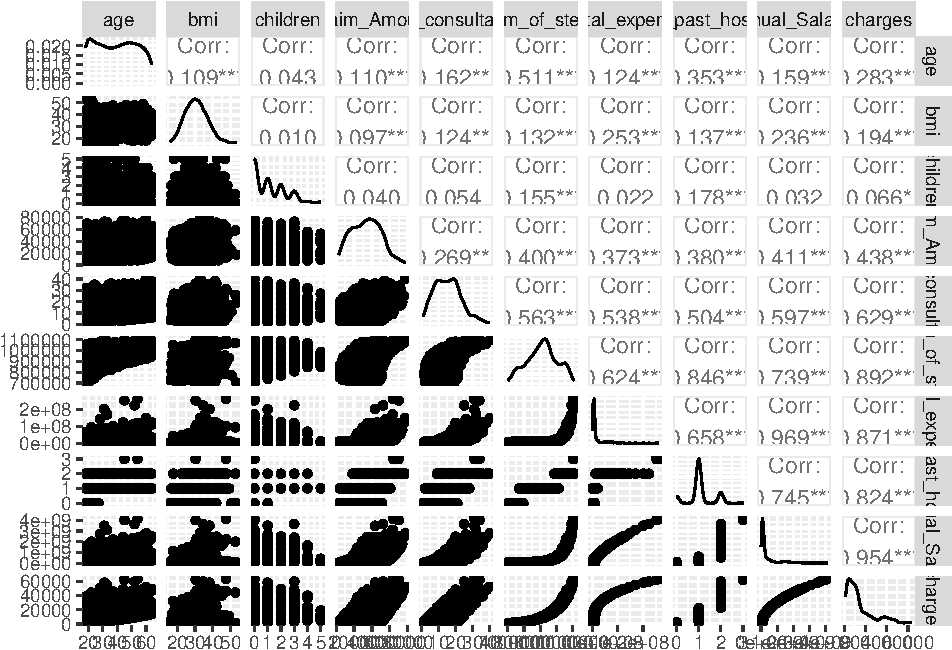
\includegraphics[keepaspectratio]{index_files/figure-latex/unnamed-chunk-4-1.pdf}}

Nótese que la variable por predecir, \texttt{charges}, parece presentar
una relación lineal con la covariable \texttt{Annual\_Salary}. Asimismo,
parece haber indicios de que resulta posible transformar las variables
\texttt{num\_of\_steps} y \texttt{Hospital\_expenditure} por funciones
logaritmo y exponcial, respectivamente, con fin que se tenga una fuerte
relación lineal entre el predictor creado y la variable por predecir.

\paragraph{Correlaciones parciales entre
covariables}\label{correlaciones-parciales-entre-covariables}

\begin{Shaded}
\begin{Highlighting}[]
\NormalTok{d.cor }\OtherTok{\textless{}{-}} \FunctionTok{cor}\NormalTok{(datos[, covariables\_numericas])}
\NormalTok{d.inv }\OtherTok{\textless{}{-}} \FunctionTok{solve}\NormalTok{(d.cor)}

\NormalTok{d.corm }\OtherTok{\textless{}{-}} \FunctionTok{sqrt}\NormalTok{(}\DecValTok{1{-}1}\SpecialCharTok{/}\FunctionTok{diag}\NormalTok{(d.inv))}
\NormalTok{pd }\OtherTok{\textless{}{-}} \FunctionTok{length}\NormalTok{(d.corm)  }


\NormalTok{d.part }\OtherTok{\textless{}{-}}\NormalTok{ d.inv}
\ControlFlowTok{for}\NormalTok{ (i }\ControlFlowTok{in} \DecValTok{1}\SpecialCharTok{:}\NormalTok{pd) \{}
  \ControlFlowTok{for}\NormalTok{ (j }\ControlFlowTok{in} \DecValTok{1}\SpecialCharTok{:}\NormalTok{(i}\DecValTok{{-}1}\NormalTok{)) \{}
\NormalTok{    d.part[i,j] }\OtherTok{\textless{}{-}} \SpecialCharTok{{-}}\NormalTok{d.inv[i,j]}\SpecialCharTok{/}\FunctionTok{sqrt}\NormalTok{(d.inv[i,i]}\SpecialCharTok{*}\NormalTok{d.inv[j,j])}
\NormalTok{  \}}
\NormalTok{  d.part[i,i] }\OtherTok{\textless{}{-}}\NormalTok{ d.corm[i]}
\NormalTok{  d.part[}\DecValTok{1}\SpecialCharTok{:}\NormalTok{(i}\DecValTok{{-}1}\NormalTok{),i] }\OtherTok{\textless{}{-}}\NormalTok{ d.part[i,}\DecValTok{1}\SpecialCharTok{:}\NormalTok{(i}\DecValTok{{-}1}\NormalTok{)]  }
\NormalTok{\}}
\NormalTok{d.part}
\end{Highlighting}
\end{Shaded}

\begin{verbatim}
##                                         age          bmi     children Claim_Amount past_consultations num_of_steps Hospital_expenditure Number_of_past_hospitalizations Anual_Salary
## age                              0.66869810  0.125138033 -0.127797419 -0.047433079       -0.032427643   0.58296028           0.30690425                     -0.02225606  -0.38460223
## bmi                              0.12513803  0.283723310  0.027431191  0.019145260        0.002848758  -0.07315332           0.03179457                     -0.01817550   0.03462513
## children                        -0.12779742  0.027431191  0.285534954 -0.007971203        0.011798696   0.14738225           0.12834583                      0.14043273  -0.17317136
## Claim_Amount                    -0.04743308  0.019145260 -0.007971203  0.439018730       -0.005991357   0.09098912          -0.01666733                      0.02309694   0.05207480
## past_consultations              -0.03242764  0.002848758  0.011798696 -0.005991357        0.630532156   0.13217102          -0.08795473                     -0.05672368   0.16244456
## num_of_steps                     0.58296028 -0.073153318  0.147382251  0.090989121        0.132171021   0.93080551          -0.49727359                      0.45898240   0.56078648
## Hospital_expenditure             0.30690425  0.031794571  0.128345835 -0.016667332       -0.087954734  -0.49727359           0.98147153                     -0.04913622   0.95773182
## Number_of_past_hospitalizations -0.02225606 -0.018175497  0.140432728  0.023096940       -0.056723682   0.45898240          -0.04913622                      0.86849267   0.13449231
## Anual_Salary                    -0.38460223  0.034625132 -0.173171362  0.052074797        0.162444557   0.56078648           0.95773182                      0.13449231   0.98774064
\end{verbatim}

\begin{Shaded}
\begin{Highlighting}[]
\NormalTok{vals\_diag }\OtherTok{\textless{}{-}} \FunctionTok{diag}\NormalTok{(d.part)}
\NormalTok{max\_col\_indices }\OtherTok{\textless{}{-}} \FunctionTok{apply}\NormalTok{(d.part, }\DecValTok{1}\NormalTok{, which.max)}
\NormalTok{idx\_ordenados }\OtherTok{\textless{}{-}} \FunctionTok{order}\NormalTok{(vals\_diag, }\AttributeTok{decreasing =} \ConstantTok{TRUE}\NormalTok{)}
\NormalTok{ordenados\_vals\_diag }\OtherTok{\textless{}{-}}\NormalTok{ vals\_diag[idx\_ordenados]}
\NormalTok{ordenados\_max\_cols }\OtherTok{\textless{}{-}}\NormalTok{ max\_col\_indices[idx\_ordenados]}

\FunctionTok{data.frame}\NormalTok{(}\AttributeTok{correlacion\_parcial =}\NormalTok{ ordenados\_vals\_diag)}
\end{Highlighting}
\end{Shaded}

\begin{verbatim}
##                                 correlacion_parcial
## Anual_Salary                              0.9877406
## Hospital_expenditure                      0.9814715
## num_of_steps                              0.9308055
## Number_of_past_hospitalizations           0.8684927
## age                                       0.6686981
## past_consultations                        0.6305322
## Claim_Amount                              0.4390187
## children                                  0.2855350
## bmi                                       0.2837233
\end{verbatim}

Note que cuatro covariables presentan correlación parcial mayor a 0.8,
en orden descendente \texttt{Anual\_Salary},
\texttt{Hospital\_expenditure}, \texttt{num\_of\_steps} y
\texttt{Number\_of\_past\_hospitalizations}. Aquellas variables son muy
explicadas por las demás (posible multicolinearidad).

\pandocbounded{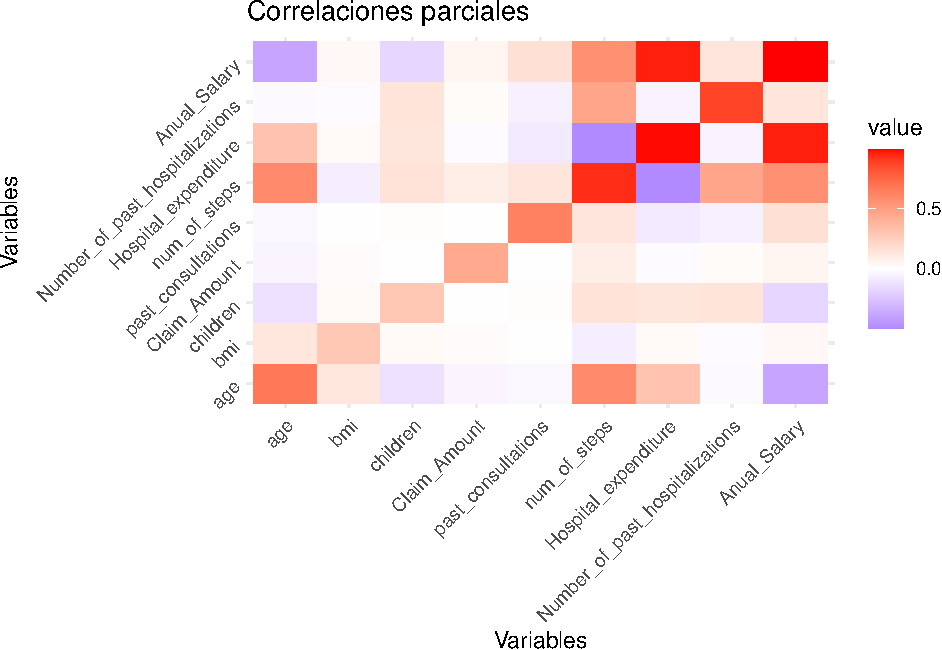
\includegraphics[keepaspectratio]{index_files/figure-latex/unnamed-chunk-7-1.pdf}}

Inspeccionemos ahora, de manera particular, las correlaciones entre
covariables

\pandocbounded{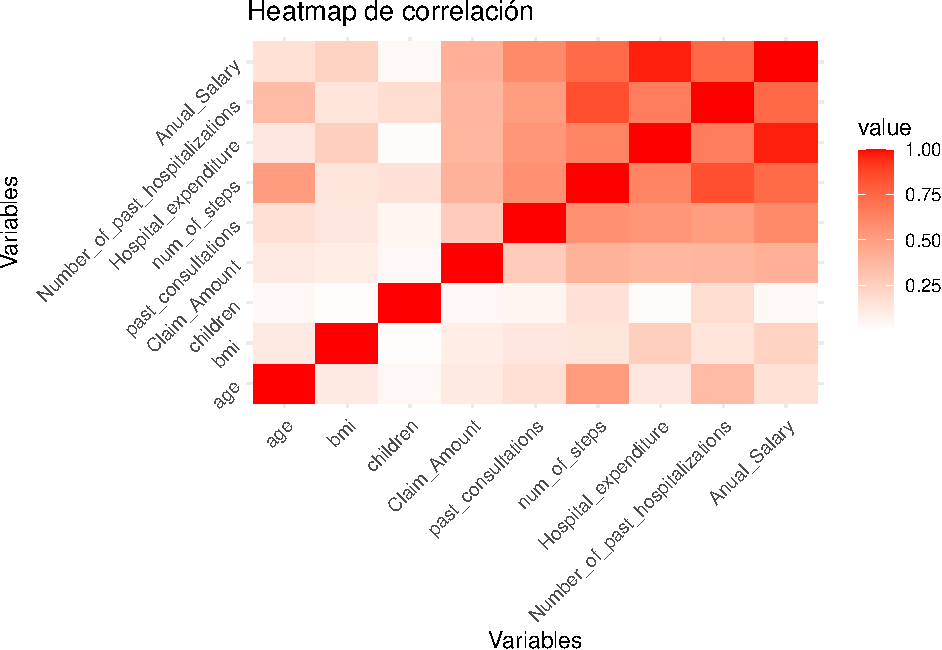
\includegraphics[keepaspectratio]{index_files/figure-latex/unnamed-chunk-8-1.pdf}}

Observamos una alta correlación entre \texttt{Anual\_Salary} y
\texttt{Hospital\_expenditure}, con un valor de 0.9692177. Asimismo,
como la variable de salario anual es más sencilla de recopilar (por
ejemplo, en una encuesta) que la de gasto de hospital, descartamos la
variable cuantitativa \texttt{Hospital\_expenditure}.

\begin{Shaded}
\begin{Highlighting}[]
\NormalTok{datos }\SpecialCharTok{|\textgreater{}}
  \FunctionTok{ggplot}\NormalTok{(}\FunctionTok{aes}\NormalTok{(}\AttributeTok{x =}\NormalTok{ Anual\_Salary, }\AttributeTok{y =}\NormalTok{ Hospital\_expenditure)) }\SpecialCharTok{+}
  \FunctionTok{geom\_point}\NormalTok{(}\AttributeTok{color =} \StringTok{"steelblue"}\NormalTok{, }\AttributeTok{alpha =} \FloatTok{0.6}\NormalTok{) }\SpecialCharTok{+}
  \FunctionTok{labs}\NormalTok{(}\AttributeTok{x =} \StringTok{"Salario anual"}\NormalTok{, }\AttributeTok{y =} \StringTok{"Gasto del hospital"}\NormalTok{) }\SpecialCharTok{+}
  \FunctionTok{theme\_minimal}\NormalTok{()}
\end{Highlighting}
\end{Shaded}

\pandocbounded{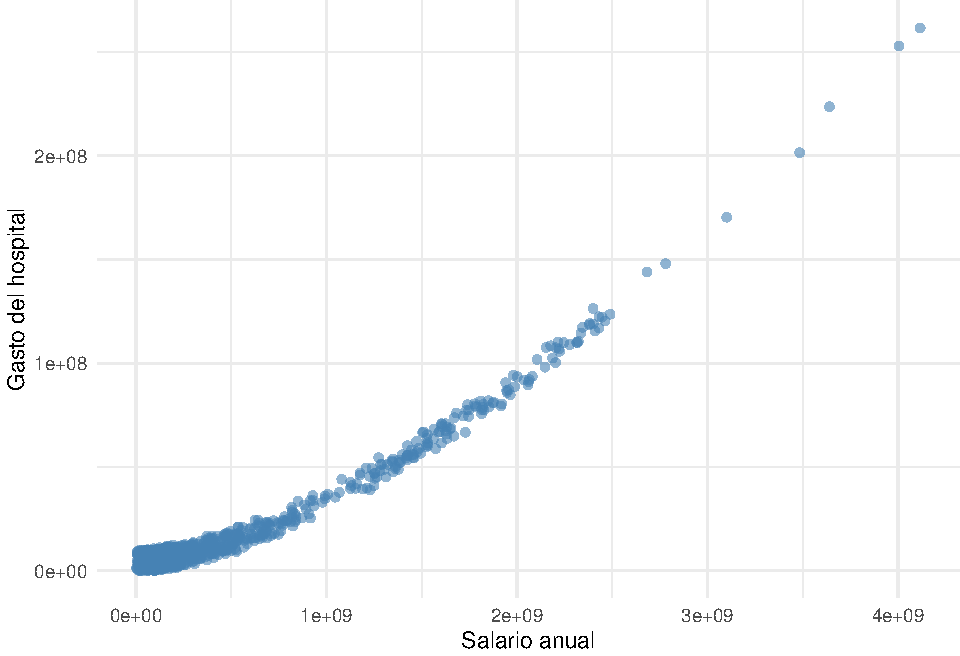
\includegraphics[keepaspectratio]{index_files/figure-latex/unnamed-chunk-9-1.pdf}}

\paragraph{\texorpdfstring{Variable cuantitativa
\texttt{num\_of\_steps}}{Variable cuantitativa num\_of\_steps}}\label{variable-cuantitativa-num_of_steps}

Inicialmente se consideró descartar la variable referente al número de
pasos que realizó el paciente en cierto día. Esto pues, a primera vista,
no se esperaría que tal información resulte relevante para el costo
final por el procedimiento médico.

Graficamos tal posible regreso contra la variable respuesta:

\begin{Shaded}
\begin{Highlighting}[]
\NormalTok{datos }\SpecialCharTok{|\textgreater{}}
  \FunctionTok{ggplot}\NormalTok{(}\FunctionTok{aes}\NormalTok{(}\AttributeTok{x =}\NormalTok{ num\_of\_steps, }\AttributeTok{y =}\NormalTok{ charges)) }\SpecialCharTok{+}
  \FunctionTok{geom\_point}\NormalTok{(}\AttributeTok{color =} \StringTok{"steelblue"}\NormalTok{, }\AttributeTok{alpha =} \FloatTok{0.6}\NormalTok{) }\SpecialCharTok{+}
  \FunctionTok{labs}\NormalTok{(}\AttributeTok{x =} \StringTok{"Número de pasos"}\NormalTok{, }\AttributeTok{y =} \StringTok{"Pago final"}\NormalTok{) }\SpecialCharTok{+}
  \FunctionTok{theme\_minimal}\NormalTok{()}
\end{Highlighting}
\end{Shaded}

\pandocbounded{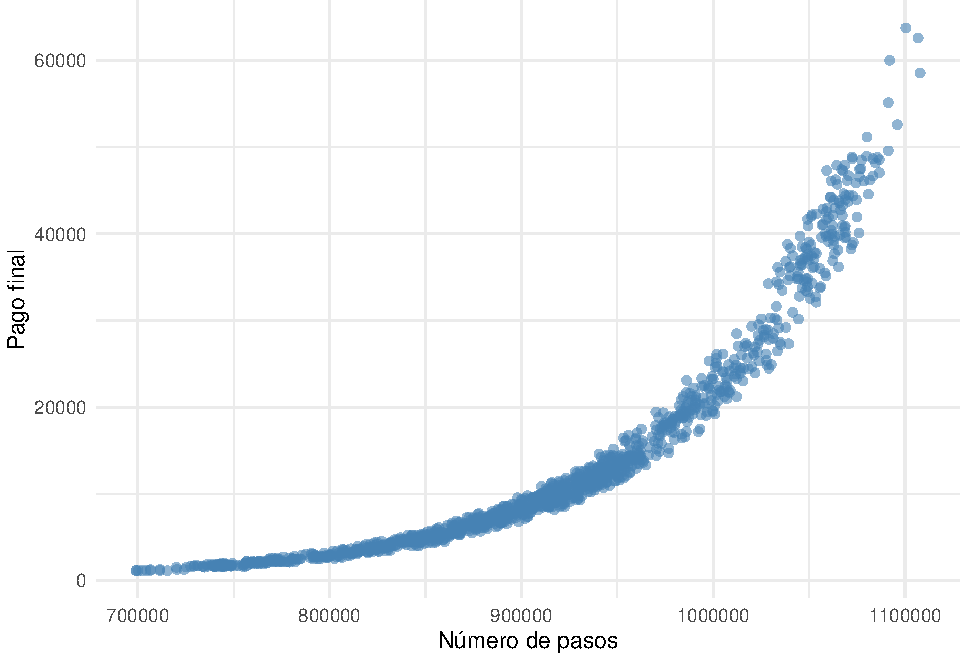
\includegraphics[keepaspectratio]{index_files/figure-latex/unnamed-chunk-10-1.pdf}}

En base a que la relación parece asemejarse a una exponencial,
graficamos la variable \texttt{num\_of\_steps} contra el logaritmo de la
variable respuesta:

\begin{Shaded}
\begin{Highlighting}[]
\NormalTok{datos }\SpecialCharTok{|\textgreater{}}
\NormalTok{  dplyr}\SpecialCharTok{::}\FunctionTok{mutate}\NormalTok{(}\AttributeTok{scaled\_rsp =} \FunctionTok{log}\NormalTok{(charges)) }\SpecialCharTok{|\textgreater{}}
  \FunctionTok{ggplot}\NormalTok{(}\FunctionTok{aes}\NormalTok{(}\AttributeTok{x =}\NormalTok{ num\_of\_steps, }\AttributeTok{y =}\NormalTok{ scaled\_rsp)) }\SpecialCharTok{+}
  \FunctionTok{geom\_point}\NormalTok{(}\AttributeTok{color =} \StringTok{"steelblue"}\NormalTok{, }\AttributeTok{alpha =} \FloatTok{0.6}\NormalTok{) }\SpecialCharTok{+}
  \FunctionTok{labs}\NormalTok{(}\AttributeTok{x =} \StringTok{"Número de pasos"}\NormalTok{, }\AttributeTok{y =} \StringTok{"Pago final"}\NormalTok{) }\SpecialCharTok{+}
  \FunctionTok{theme\_minimal}\NormalTok{()}
\end{Highlighting}
\end{Shaded}

\pandocbounded{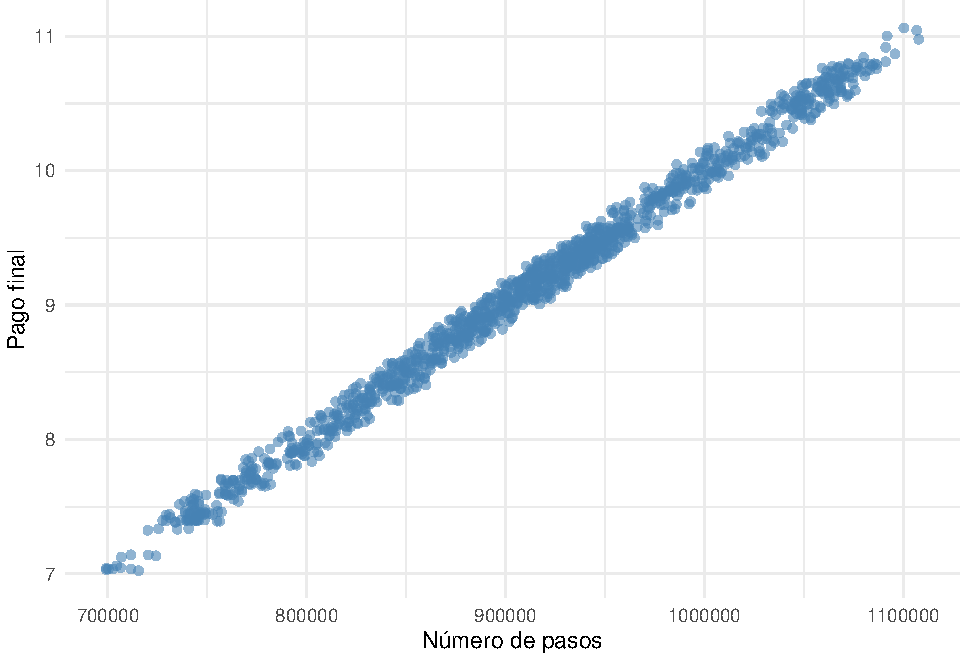
\includegraphics[keepaspectratio]{index_files/figure-latex/unnamed-chunk-11-1.pdf}}

En base a que aquella relación parece ser \emph{aproximadamente} lineal,
optamos por no descartar la variable cuantitativa
\texttt{num\_of\_steps}.

\paragraph{\texorpdfstring{Variable cuantitativa
\texttt{num\_of\_steps}}{Variable cuantitativa num\_of\_steps}}\label{variable-cuantitativa-num_of_steps-1}

\begin{Shaded}
\begin{Highlighting}[]
\NormalTok{datos }\SpecialCharTok{|\textgreater{}}
  \FunctionTok{ggplot}\NormalTok{(}\FunctionTok{aes}\NormalTok{(}\AttributeTok{x =}\NormalTok{ num\_of\_steps, }\AttributeTok{y =}\NormalTok{ charges)) }\SpecialCharTok{+}
  \FunctionTok{geom\_point}\NormalTok{(}\AttributeTok{color =} \StringTok{"steelblue"}\NormalTok{, }\AttributeTok{alpha =} \FloatTok{0.6}\NormalTok{) }\SpecialCharTok{+}
  \FunctionTok{labs}\NormalTok{(}\AttributeTok{x =} \StringTok{"Número de pasos"}\NormalTok{, }\AttributeTok{y =} \StringTok{"Pago final"}\NormalTok{) }\SpecialCharTok{+}
  \FunctionTok{theme\_minimal}\NormalTok{()}
\end{Highlighting}
\end{Shaded}

\pandocbounded{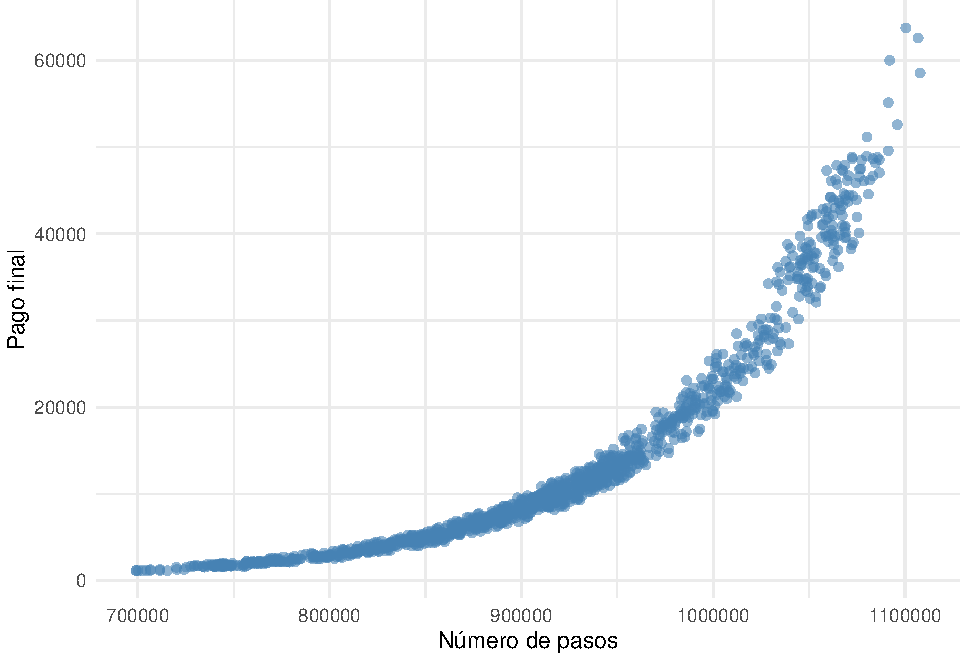
\includegraphics[keepaspectratio]{index_files/figure-latex/unnamed-chunk-12-1.pdf}}

\paragraph{\texorpdfstring{Variable cuantitativa
\texttt{age}}{Variable cuantitativa age}}\label{variable-cuantitativa-age}

\begin{Shaded}
\begin{Highlighting}[]
\NormalTok{datos }\SpecialCharTok{|\textgreater{}}
  \FunctionTok{ggplot}\NormalTok{(}\FunctionTok{aes}\NormalTok{(}\AttributeTok{x =}\NormalTok{ age, }\AttributeTok{y =}\NormalTok{ charges)) }\SpecialCharTok{+}
  \FunctionTok{geom\_point}\NormalTok{(}\AttributeTok{color =} \StringTok{"steelblue"}\NormalTok{, }\AttributeTok{alpha =} \FloatTok{0.6}\NormalTok{) }\SpecialCharTok{+}
  \FunctionTok{labs}\NormalTok{(}\AttributeTok{x =} \StringTok{"Edad"}\NormalTok{, }\AttributeTok{y =} \StringTok{"Pago final"}\NormalTok{) }\SpecialCharTok{+}
  \FunctionTok{theme\_minimal}\NormalTok{()}
\end{Highlighting}
\end{Shaded}

\pandocbounded{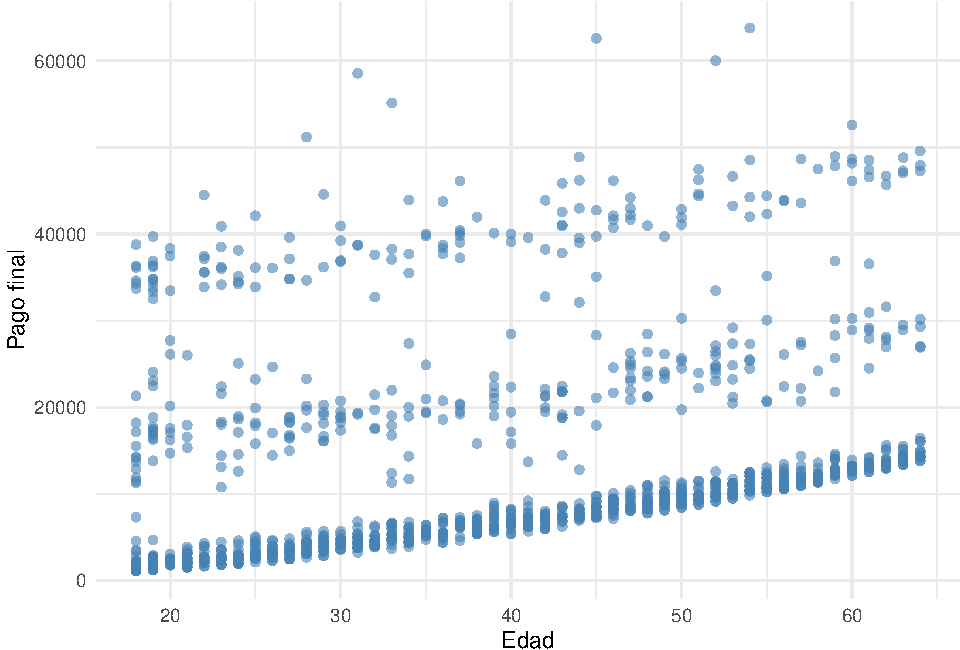
\includegraphics[keepaspectratio]{index_files/figure-latex/unnamed-chunk-13-1.pdf}}

\paragraph{\texorpdfstring{Variable cuantitativa
\texttt{bmi}}{Variable cuantitativa bmi}}\label{variable-cuantitativa-bmi}

\begin{Shaded}
\begin{Highlighting}[]
\NormalTok{datos }\SpecialCharTok{|\textgreater{}}
  \FunctionTok{ggplot}\NormalTok{(}\FunctionTok{aes}\NormalTok{(}\AttributeTok{x =}\NormalTok{ bmi, }\AttributeTok{y =}\NormalTok{ charges)) }\SpecialCharTok{+}
  \FunctionTok{geom\_point}\NormalTok{(}\AttributeTok{color =} \StringTok{"steelblue"}\NormalTok{, }\AttributeTok{alpha =} \FloatTok{0.6}\NormalTok{) }\SpecialCharTok{+}
  \FunctionTok{labs}\NormalTok{(}\AttributeTok{x =} \StringTok{"Índice de masa corporal"}\NormalTok{, }\AttributeTok{y =} \StringTok{"Pago final"}\NormalTok{) }\SpecialCharTok{+}
  \FunctionTok{theme\_minimal}\NormalTok{()}
\end{Highlighting}
\end{Shaded}

\pandocbounded{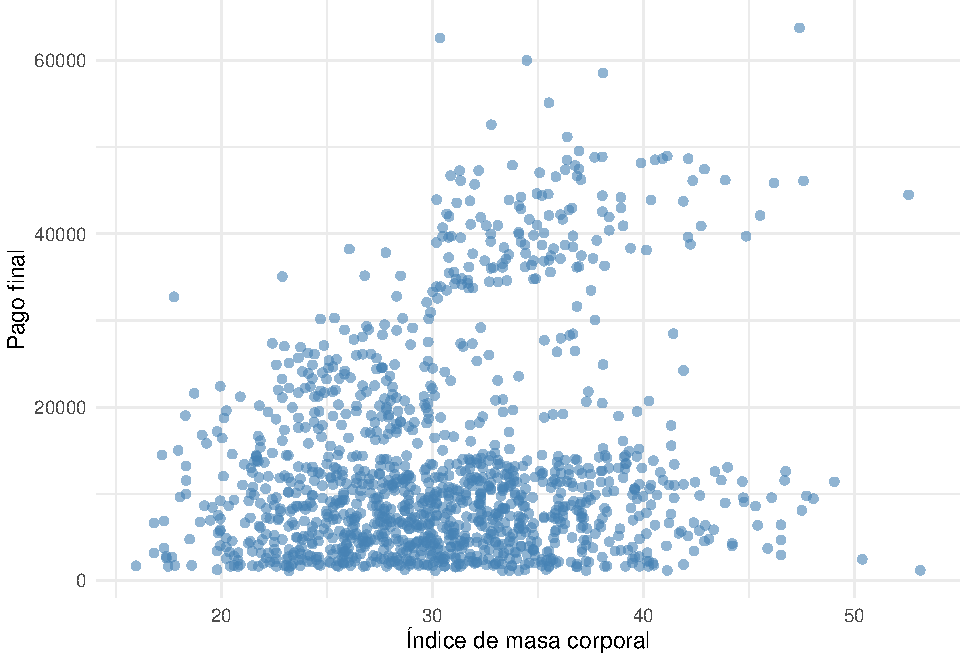
\includegraphics[keepaspectratio]{index_files/figure-latex/unnamed-chunk-14-1.pdf}}

\paragraph{\texorpdfstring{Variable cuantitativa
\texttt{children}}{Variable cuantitativa children}}\label{variable-cuantitativa-children}

\begin{Shaded}
\begin{Highlighting}[]
\NormalTok{datos }\SpecialCharTok{|\textgreater{}}
  \FunctionTok{ggplot}\NormalTok{(}\FunctionTok{aes}\NormalTok{(}\AttributeTok{x =}\NormalTok{ children, }\AttributeTok{y =}\NormalTok{ charges)) }\SpecialCharTok{+}
  \FunctionTok{geom\_point}\NormalTok{(}\AttributeTok{color =} \StringTok{"steelblue"}\NormalTok{, }\AttributeTok{alpha =} \FloatTok{0.6}\NormalTok{) }\SpecialCharTok{+}
  \FunctionTok{labs}\NormalTok{(}\AttributeTok{x =} \StringTok{"Número de hijos"}\NormalTok{, }\AttributeTok{y =} \StringTok{"Pago final"}\NormalTok{) }\SpecialCharTok{+}
  \FunctionTok{theme\_minimal}\NormalTok{()}
\end{Highlighting}
\end{Shaded}

\pandocbounded{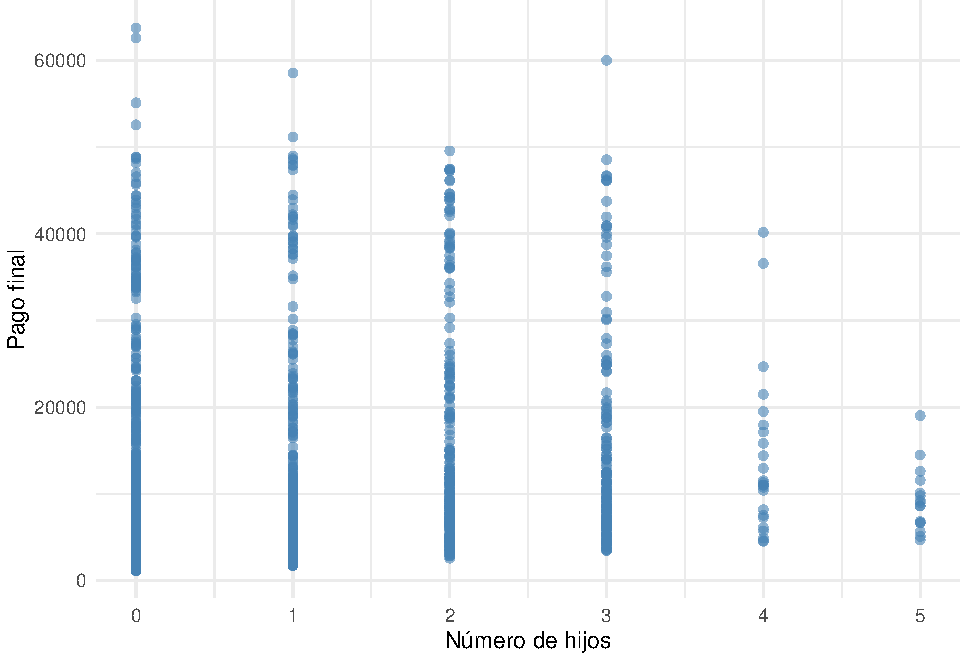
\includegraphics[keepaspectratio]{index_files/figure-latex/unnamed-chunk-15-1.pdf}}

\paragraph{\texorpdfstring{Variable cuantitativa
\texttt{past\_consultations}}{Variable cuantitativa past\_consultations}}\label{variable-cuantitativa-past_consultations}

\begin{Shaded}
\begin{Highlighting}[]
\NormalTok{datos }\SpecialCharTok{|\textgreater{}}
  \FunctionTok{ggplot}\NormalTok{(}\FunctionTok{aes}\NormalTok{(}\AttributeTok{x =}\NormalTok{ past\_consultations, }\AttributeTok{y =}\NormalTok{ charges)) }\SpecialCharTok{+}
  \FunctionTok{geom\_point}\NormalTok{(}\AttributeTok{color =} \StringTok{"steelblue"}\NormalTok{, }\AttributeTok{alpha =} \FloatTok{0.6}\NormalTok{) }\SpecialCharTok{+}
  \FunctionTok{labs}\NormalTok{(}\AttributeTok{x =} \StringTok{"Número de procedimientos pasados"}\NormalTok{, }\AttributeTok{y =} \StringTok{"Pago final"}\NormalTok{) }\SpecialCharTok{+}
  \FunctionTok{theme\_minimal}\NormalTok{()}
\end{Highlighting}
\end{Shaded}

\pandocbounded{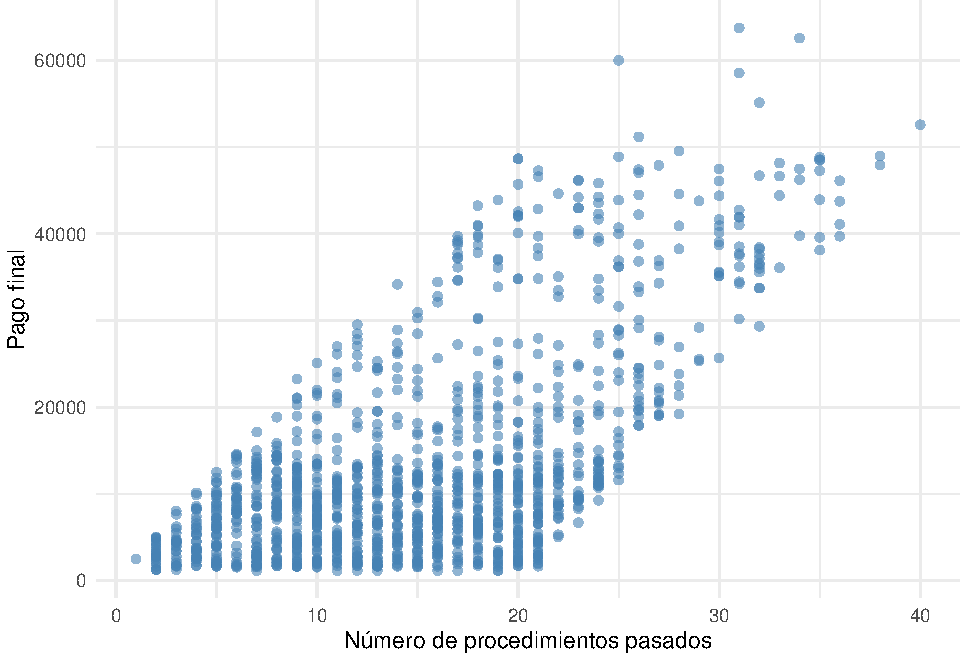
\includegraphics[keepaspectratio]{index_files/figure-latex/unnamed-chunk-16-1.pdf}}

Descartamos la variable cuantitativa \texttt{children}, pues, en base a
este simple análisis inicial, no parece indicar algún de tipo de
relación lineal con la variable por predecir. Es más, su gráfico de
dispersión parece sugerir que consideremos a la variable
\texttt{children} como cualitativa.

\paragraph{Variables categóricas}\label{variables-categuxf3ricas}

Para el filtro de variables categóricas, descartaremos aquella para la
cual las distribuciones de la variable respuesta, respecto a los valores
de aquella variable categórica sean relativamente similares.

\paragraph{\texorpdfstring{Variable cualitativa
\texttt{region}}{Variable cualitativa region}}\label{variable-cualitativa-region}

Inspeccionamos la distribución de la variable respuesta, respecto a los
valores de la variable categórica \texttt{region}.

\begin{Shaded}
\begin{Highlighting}[]
\NormalTok{datos }\SpecialCharTok{|\textgreater{}}
  \FunctionTok{ggplot}\NormalTok{(}\FunctionTok{aes}\NormalTok{(}\AttributeTok{x =}\NormalTok{ charges, }\AttributeTok{color =}\NormalTok{ region, }\AttributeTok{fill =}\NormalTok{ region)) }\SpecialCharTok{+}
    \FunctionTok{geom\_density}\NormalTok{(}\AttributeTok{alpha =} \FloatTok{0.4}\NormalTok{) }\SpecialCharTok{+}
    \FunctionTok{labs}\NormalTok{(}
      \AttributeTok{title =} \StringTok{"Densidad de \textquotesingle{}charges\textquotesingle{} para cada categoría de \textquotesingle{}region\textquotesingle{}"}\NormalTok{,}
      \AttributeTok{x =} \StringTok{"charges"}\NormalTok{,}
      \AttributeTok{y =} \StringTok{"Densidad"}
\NormalTok{    ) }\SpecialCharTok{+}
    \FunctionTok{theme\_minimal}\NormalTok{()}
\end{Highlighting}
\end{Shaded}

\pandocbounded{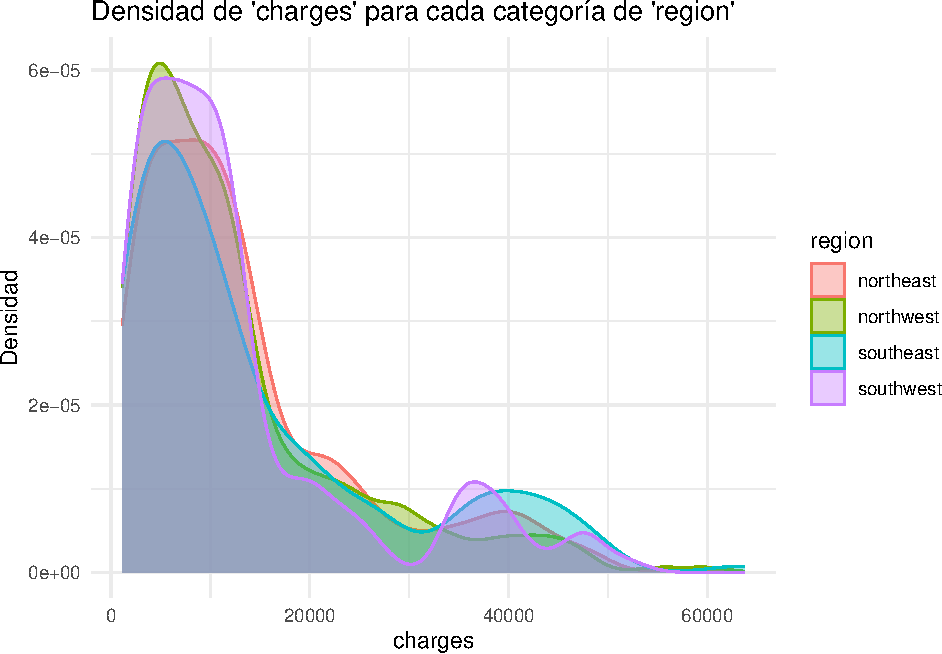
\includegraphics[keepaspectratio]{index_files/figure-latex/unnamed-chunk-17-1.pdf}}

En base a que aquellas funciones densidad no presentan una difencia
resaltante, descartaremos la variable \texttt{region}. De esa manera,
las variables cualitativas que emplearemos para esta investigación son
solo \texttt{sex} y \texttt{smoker}.

\paragraph{Variables finales}\label{variables-finales}

\begin{itemize}
\tightlist
\item
  Variables cualitativas:

  \begin{itemize}
  \tightlist
  \item
    \texttt{sex}
  \item
    \texttt{smoker}
  \end{itemize}
\item
  Variables cuantitativas:

  \begin{itemize}
  \tightlist
  \item
    \texttt{age}
  \item
    \texttt{bmi}
  \item
    \texttt{Claim\_Amount}
  \item
    \texttt{past\_consultations}
  \item
    \texttt{num\_of\_steps}
  \item
    \texttt{Number\_of\_past\_hospitalizations}
  \item
    \texttt{Anual\_Salary}
  \item
    \texttt{charges} (\textbf{variable respuesta})
  \end{itemize}
\end{itemize}

Para limitarnos a 500 filas, según la restricción de este proyecto,
realizaremos un muestreo:

\begin{Shaded}
\begin{Highlighting}[]
\NormalTok{obs }\OtherTok{\textless{}{-}}\NormalTok{ datos }\SpecialCharTok{|\textgreater{}}
\NormalTok{  dplyr}\SpecialCharTok{::}\FunctionTok{select}\NormalTok{(}
\NormalTok{    sex,}
\NormalTok{    smoker,}
\NormalTok{    age,}
\NormalTok{    bmi,}
\NormalTok{    Claim\_Amount,}
\NormalTok{    past\_consultations,}
\NormalTok{    num\_of\_steps,}
\NormalTok{    Number\_of\_past\_hospitalizations,}
\NormalTok{    Anual\_Salary,}
\NormalTok{    charges}
\NormalTok{  )}

\FunctionTok{set.seed}\NormalTok{(}\DecValTok{1234}\NormalTok{)}
\NormalTok{obs }\OtherTok{\textless{}{-}}\NormalTok{ dplyr}\SpecialCharTok{::}\FunctionTok{sample\_n}\NormalTok{(obs, }\DecValTok{500}\NormalTok{)}

\NormalTok{openxlsx}\SpecialCharTok{::}\FunctionTok{write.xlsx}\NormalTok{(obs, }\StringTok{\textquotesingle{}./datos.xlsx\textquotesingle{}}\NormalTok{)}
\end{Highlighting}
\end{Shaded}

\subsubsection{Modelamiento}\label{modelamiento}

Note que los tipos de datos de las covariables son adecuadas. En
particular, las funciones por emplear se encargarán de la conversión
numérica a las covariables categóricas \texttt{age} y \texttt{sex}.

\begin{Shaded}
\begin{Highlighting}[]
\NormalTok{dplyr}\SpecialCharTok{::}\FunctionTok{glimpse}\NormalTok{(obs)}
\end{Highlighting}
\end{Shaded}

\begin{verbatim}
## Rows: 500
## Columns: 10
## $ sex                             <chr> "male", "female", "male", "female", "male", "male", "female", "male", "female", "female", "female", "female", "female", "male", "female", "male", "male", "fem~
## $ smoker                          <chr> "no", "no", "yes", "no", "no", "no", "no", "no", "no", "no", "no", "no", "no", "yes", "no", "no", "no", "no", "no", "no", "yes", "no", "yes", "no", "no", "no"~
## $ age                             <dbl> 28, 40, 33, 48, 63, 48, 59, 38, 63, 22, 60, 54, 36, 56, 62, 27, 21, 47, 18, 46, 45, 64, 46, 27, 38, 51, 63, 47, 63, 24, 52, 42, 50, 30, 27, 24, 44, 33, 49, 37~
## $ bmi                             <dbl> 33.820, 41.420, 27.100, 28.880, 31.445, 34.300, 32.395, 34.700, 31.800, 24.300, 25.840, 31.900, 29.920, 26.695, 25.000, 30.300, 23.750, 24.320, 33.660, 28.050~
## $ Claim_Amount                    <dbl> 24107.866, 27534.303, 39952.923, 45755.609, 34045.546, 36944.415, 44301.816, 8821.036, 26903.710, 5288.527, 64241.695, 41178.475, 10662.504, 24067.406, 28821.~
## $ past_consultations              <dbl> 18, 15, 27, 24, 14, 18, 18, 12, 11, 8, 14, 24, 9, 11, 7, 17, 16, 7, 11, 18, 31, 16, 25, 22, 18, 6, 19, 12, 12, 4, 19, 13, 21, 3, 5, 11, 24, 17, 5, 21, 21, 19,~
## $ num_of_steps                    <dbl> 983349, 1031312, 996320, 912509, 953355, 926940, 940460, 880463, 954102, 764144, 1028596, 919493, 854473, 1001767, 955589, 849404, 801695, 914552, 700250, 889~
## $ Number_of_past_hospitalizations <dbl> 1, 2, 1, 1, 1, 1, 1, 1, 1, 0, 2, 1, 1, 2, 1, 1, 1, 1, 0, 1, 2, 1, 2, 1, 1, 1, 1, 1, 2, 0, 2, 1, 1, 1, 1, 0, 2, 1, 1, 1, 1, 2, 1, 0, 2, 1, 0, 1, 1, 1, 1, 1, 2,~
## $ Anual_Salary                    <dbl> 481649496, 869010594, 453727467, 178469707, 233696716, 101378109, 289788380, 85599131, 194691807, 83114999, 933206179, 149223189, 83254162, 749221179, 1989239~
## $ charges                         <dbl> 19673.336, 28476.735, 19040.876, 9249.495, 13974.456, 9563.029, 14590.632, 6082.405, 13880.949, 2150.469, 28923.137, 10928.849, 4889.037, 26109.329, 13451.122~
\end{verbatim}

Comencemos definiendo algunas funciones auxliares en el análisis y
modelamiento.

\begin{Shaded}
\begin{Highlighting}[]
\NormalTok{sum.lm }\OtherTok{\textless{}{-}} \ControlFlowTok{function}\NormalTok{(lmod) \{}
\NormalTok{  summ }\OtherTok{\textless{}{-}} \FunctionTok{summary}\NormalTok{(lmod)}
\NormalTok{  ci }\OtherTok{\textless{}{-}} \FunctionTok{confint}\NormalTok{(lmod)}
\NormalTok{  summ}\SpecialCharTok{$}\NormalTok{coefficients }\OtherTok{\textless{}{-}} \FunctionTok{cbind}\NormalTok{(}
\NormalTok{    summ}\SpecialCharTok{$}\NormalTok{coefficients[,}\DecValTok{1}\NormalTok{],}
\NormalTok{    ci,summ}\SpecialCharTok{$}\NormalTok{coefficients[,}\DecValTok{2}\SpecialCharTok{:}\DecValTok{4}\NormalTok{]}
\NormalTok{  )}
  \FunctionTok{return}\NormalTok{(summ)}
\NormalTok{\}}

\NormalTok{extraer\_estadistica\_f }\OtherTok{\textless{}{-}} \ControlFlowTok{function}\NormalTok{(modelo) \{}
  \FunctionTok{return}\NormalTok{(}\FunctionTok{summary}\NormalTok{(modelo)}\SpecialCharTok{$}\NormalTok{fstatistic[}\DecValTok{1}\NormalTok{])}
\NormalTok{\}}

\NormalTok{obtener\_p\_valor\_de\_estadistica\_f }\OtherTok{\textless{}{-}} \ControlFlowTok{function}\NormalTok{(modelo) \{}
\NormalTok{  s }\OtherTok{\textless{}{-}} \FunctionTok{summary}\NormalTok{(modelo)}

\NormalTok{  fval }\OtherTok{\textless{}{-}}\NormalTok{ s}\SpecialCharTok{$}\NormalTok{fstatistic[}\StringTok{"value"}\NormalTok{]}
\NormalTok{  df1 }\OtherTok{\textless{}{-}}\NormalTok{ s}\SpecialCharTok{$}\NormalTok{fstatistic[}\StringTok{"numdf"}\NormalTok{]}
\NormalTok{  df2 }\OtherTok{\textless{}{-}}\NormalTok{ s}\SpecialCharTok{$}\NormalTok{fstatistic[}\StringTok{"dendf"}\NormalTok{]}

  \FunctionTok{return}\NormalTok{(}\FunctionTok{pf}\NormalTok{(fval, df1, df2, }\AttributeTok{lower.tail =} \ConstantTok{FALSE}\NormalTok{))}
\NormalTok{\}}

\NormalTok{extraer\_info\_t\_student }\OtherTok{\textless{}{-}} \ControlFlowTok{function}\NormalTok{(modelo) \{}
\NormalTok{  df }\OtherTok{\textless{}{-}} \FunctionTok{as.data.frame}\NormalTok{(}\FunctionTok{summary}\NormalTok{(modelo)}\SpecialCharTok{$}\NormalTok{coefficients)}
\NormalTok{  df }\OtherTok{\textless{}{-}}\NormalTok{ df[}\SpecialCharTok{{-}}\DecValTok{1}\NormalTok{, }\FunctionTok{c}\NormalTok{(}\SpecialCharTok{{-}}\DecValTok{1}\NormalTok{, }\SpecialCharTok{{-}}\DecValTok{2}\NormalTok{)]}

\NormalTok{  df}\SpecialCharTok{$}\NormalTok{es\_significativo }\OtherTok{\textless{}{-}}\NormalTok{ df[, }\DecValTok{2}\NormalTok{] }\SpecialCharTok{\textless{}} \FloatTok{0.05}
  \FunctionTok{return}\NormalTok{(df)}
\NormalTok{\}}

\CommentTok{\# Implementación básica de la función car::ncvTest, debido a que}
\CommentTok{\# no me funciona descargar aquella librería.}
\NormalTok{ncvTest }\OtherTok{\textless{}{-}} \ControlFlowTok{function}\NormalTok{(modelo, }\AttributeTok{variable =} \ConstantTok{NULL}\NormalTok{) \{}
  \CommentTok{\# Verifica si el modelo es lineal}
  \ControlFlowTok{if}\NormalTok{ (}\SpecialCharTok{!}\FunctionTok{inherits}\NormalTok{(modelo, }\StringTok{"lm"}\NormalTok{)) }\FunctionTok{stop}\NormalTok{(}\StringTok{"El modelo debe ser de clase \textquotesingle{}lm\textquotesingle{}"}\NormalTok{)}
  
  \CommentTok{\# Extrae los residuos y los valores ajustados}
\NormalTok{  residuos }\OtherTok{\textless{}{-}} \FunctionTok{residuals}\NormalTok{(modelo)}
\NormalTok{  ajustados }\OtherTok{\textless{}{-}} \FunctionTok{fitted}\NormalTok{(modelo)}
  
  \CommentTok{\# Selecciona la variable de prueba}
  \ControlFlowTok{if}\NormalTok{ (}\FunctionTok{is.null}\NormalTok{(variable)) \{}
\NormalTok{    z }\OtherTok{\textless{}{-}}\NormalTok{ ajustados  }\CommentTok{\# por defecto, se usa contra los valores ajustados}
\NormalTok{  \} }\ControlFlowTok{else}\NormalTok{ \{}
\NormalTok{    datos\_modelo }\OtherTok{\textless{}{-}} \FunctionTok{model.frame}\NormalTok{(modelo)}
\NormalTok{    z }\OtherTok{\textless{}{-}}\NormalTok{ datos\_modelo[[variable]]}
    \ControlFlowTok{if}\NormalTok{ (}\FunctionTok{is.null}\NormalTok{(z)) }\FunctionTok{stop}\NormalTok{(}\StringTok{"Variable no encontrada en el marco del modelo"}\NormalTok{)}
\NormalTok{  \}}
  
  \CommentTok{\# Calcula la estadística de prueba}
\NormalTok{  score }\OtherTok{\textless{}{-}} \FunctionTok{sum}\NormalTok{(residuos}\SpecialCharTok{\^{}}\DecValTok{2} \SpecialCharTok{*}\NormalTok{ z)}
\NormalTok{  informacion }\OtherTok{\textless{}{-}} \FunctionTok{sum}\NormalTok{((residuos }\SpecialCharTok{*}\NormalTok{ z)}\SpecialCharTok{\^{}}\DecValTok{2}\NormalTok{)}
\NormalTok{  estadistico }\OtherTok{\textless{}{-}}\NormalTok{ score}\SpecialCharTok{\^{}}\DecValTok{2} \SpecialCharTok{/}\NormalTok{ informacion}
  
  \CommentTok{\# Calcula el valor p}
\NormalTok{  valor\_p }\OtherTok{\textless{}{-}} \DecValTok{1} \SpecialCharTok{{-}} \FunctionTok{pchisq}\NormalTok{(estadistico, }\AttributeTok{df =} \DecValTok{1}\NormalTok{)}
  
  \CommentTok{\# Devuelve como objeto de prueba}
\NormalTok{  resultado }\OtherTok{\textless{}{-}} \FunctionTok{list}\NormalTok{(}\AttributeTok{statistic =}\NormalTok{ estadistico, }\AttributeTok{p.value =}\NormalTok{ valor\_p)}
  \FunctionTok{class}\NormalTok{(resultado) }\OtherTok{\textless{}{-}} \StringTok{"htest"}
  \FunctionTok{return}\NormalTok{(resultado)}
\NormalTok{\}}

\NormalTok{resaltar\_n\_puntos\_con\_mayor\_apalancamiento }\OtherTok{\textless{}{-}} \ControlFlowTok{function}\NormalTok{(modelo, }\AttributeTok{n =} \DecValTok{10}\NormalTok{) \{}
\NormalTok{  graficos }\OtherTok{\textless{}{-}} \FunctionTok{list}\NormalTok{()}

\NormalTok{  observaciones }\OtherTok{\textless{}{-}}\NormalTok{ modelo}\SpecialCharTok{$}\NormalTok{model[[}\DecValTok{1}\NormalTok{]]}
\NormalTok{  estimaciones }\OtherTok{\textless{}{-}}\NormalTok{ modelo}\SpecialCharTok{$}\NormalTok{fitted.values}

\NormalTok{  graficos}\SpecialCharTok{$}\NormalTok{est\_vs\_obs }\OtherTok{\textless{}{-}} \ControlFlowTok{function}\NormalTok{ () \{}
\NormalTok{    abs\_resid }\OtherTok{\textless{}{-}} \FunctionTok{abs}\NormalTok{(observaciones }\SpecialCharTok{{-}}\NormalTok{ estimaciones)}
\NormalTok{    top10\_idx }\OtherTok{\textless{}{-}} \FunctionTok{order}\NormalTok{(abs\_resid, }\AttributeTok{decreasing =} \ConstantTok{TRUE}\NormalTok{)[}\DecValTok{1}\SpecialCharTok{:}\NormalTok{n]}

    \FunctionTok{plot}\NormalTok{(}
\NormalTok{      estimaciones, }
\NormalTok{      observaciones,}
      \AttributeTok{col =} \FunctionTok{ifelse}\NormalTok{(}\DecValTok{1}\SpecialCharTok{:}\FunctionTok{length}\NormalTok{(observaciones) }\SpecialCharTok{\%in\%}\NormalTok{ top10\_idx, }\StringTok{"red"}\NormalTok{, }\StringTok{"black"}\NormalTok{),}
      \AttributeTok{pch =} \DecValTok{19}\NormalTok{,}
      \AttributeTok{xlab =} \StringTok{"estimaciones"}\NormalTok{,}
      \AttributeTok{ylab =} \StringTok{"observaciones"}
\NormalTok{    )}
    \FunctionTok{abline}\NormalTok{(}\AttributeTok{a =} \DecValTok{0}\NormalTok{, }\AttributeTok{b =} \DecValTok{1}\NormalTok{, }\AttributeTok{col =} \StringTok{"blue"}\NormalTok{, }\AttributeTok{lty =} \DecValTok{2}\NormalTok{)}
    \FunctionTok{abline}\NormalTok{(}\FunctionTok{lm}\NormalTok{(observaciones }\SpecialCharTok{\textasciitilde{}}\NormalTok{ estimaciones), }\AttributeTok{col =} \StringTok{"darkgreen"}\NormalTok{, }\AttributeTok{lwd =} \DecValTok{2}\NormalTok{)}
\NormalTok{  \}}

\NormalTok{  graficos}\SpecialCharTok{$}\NormalTok{est\_vs\_res }\OtherTok{\textless{}{-}} \ControlFlowTok{function}\NormalTok{ () \{}
\NormalTok{    residuos }\OtherTok{\textless{}{-}}\NormalTok{ modelo}\SpecialCharTok{$}\NormalTok{residuals}
\NormalTok{    abs\_resid }\OtherTok{\textless{}{-}} \FunctionTok{abs}\NormalTok{(residuos)}

\NormalTok{    top10\_idx }\OtherTok{\textless{}{-}} \FunctionTok{order}\NormalTok{(abs\_resid, }\AttributeTok{decreasing =} \ConstantTok{TRUE}\NormalTok{)[}\DecValTok{1}\SpecialCharTok{:}\NormalTok{n]}

    \FunctionTok{plot}\NormalTok{(}
\NormalTok{      estimaciones, }
\NormalTok{      residuos,}
      \AttributeTok{col =} \FunctionTok{ifelse}\NormalTok{(}\DecValTok{1}\SpecialCharTok{:}\FunctionTok{length}\NormalTok{(residuos) }\SpecialCharTok{\%in\%}\NormalTok{ top10\_idx, }\StringTok{"red"}\NormalTok{, }\StringTok{"black"}\NormalTok{),}
      \AttributeTok{pch =} \DecValTok{19}\NormalTok{,}
      \AttributeTok{xlab =} \StringTok{"estimaciones"}\NormalTok{,}
      \AttributeTok{ylab =} \StringTok{"residuos"}
\NormalTok{    )}
    \FunctionTok{abline}\NormalTok{(}\AttributeTok{h =} \DecValTok{0}\NormalTok{, }\AttributeTok{lty =} \DecValTok{2}\NormalTok{, }\AttributeTok{col =} \StringTok{"blue"}\NormalTok{)}
\NormalTok{  \}}

  \FunctionTok{return}\NormalTok{(graficos)}
\NormalTok{\}}

\NormalTok{calcular\_rse }\OtherTok{\textless{}{-}} \ControlFlowTok{function}\NormalTok{(modelo) \{}
\NormalTok{  k }\OtherTok{\textless{}{-}} \FunctionTok{length}\NormalTok{(modelo}\SpecialCharTok{$}\NormalTok{coefficients) }\SpecialCharTok{{-}} \DecValTok{1}
\NormalTok{  SSE }\OtherTok{\textless{}{-}} \FunctionTok{sum}\NormalTok{(modelo}\SpecialCharTok{$}\NormalTok{residuals}\SpecialCharTok{**}\DecValTok{2}\NormalTok{)}
\NormalTok{  num\_obs }\OtherTok{\textless{}{-}} \FunctionTok{length}\NormalTok{(modelo}\SpecialCharTok{$}\NormalTok{residuals)}

  \FunctionTok{return}\NormalTok{(}\FunctionTok{sqrt}\NormalTok{(SSE}\SpecialCharTok{/}\NormalTok{(num\_obs }\SpecialCharTok{{-}}\NormalTok{ (}\DecValTok{1}\SpecialCharTok{+}\NormalTok{k))))}
\NormalTok{\}}
\end{Highlighting}
\end{Shaded}

\paragraph{Modelo completo}\label{modelo-completo}

\begin{Shaded}
\begin{Highlighting}[]
\NormalTok{modelo\_completo }\OtherTok{\textless{}{-}} \FunctionTok{lm}\NormalTok{(charges }\SpecialCharTok{\textasciitilde{}}\NormalTok{ ., obs)}
\FunctionTok{sum.lm}\NormalTok{(modelo\_completo)}
\end{Highlighting}
\end{Shaded}

\begin{verbatim}
## 
## Call:
## lm(formula = charges ~ ., data = obs)
## 
## Residuals:
##     Min      1Q  Median      3Q     Max 
## -3574.8  -728.0  -121.6   631.4  3762.3 
## 
## Coefficients:
##                                                 2.5 %     97.5 % Std. Error t value Pr(>|t|)    
## (Intercept)                     -4.223e+04 -4.430e+04 -4.016e+04  1.055e+03 -40.029  < 2e-16 ***
## sexmale                          1.018e+02 -9.310e+01  2.967e+02  9.919e+01   1.026    0.305    
## smokeryes                        3.807e+02 -1.072e+02  8.686e+02  2.483e+02   1.533    0.126    
## age                             -2.649e+01 -3.670e+01 -1.628e+01  5.196e+00  -5.097 4.93e-07 ***
## bmi                             -1.680e+01 -3.465e+01  1.046e+00  9.083e+00  -1.850    0.065 .  
## Claim_Amount                     2.238e-03 -4.649e-03  9.125e-03  3.505e-03   0.639    0.523    
## past_consultations               7.868e-01 -1.567e+01  1.725e+01  8.378e+00   0.094    0.925    
## num_of_steps                     5.771e-02  5.491e-02  6.051e-02  1.427e-03  40.434  < 2e-16 ***
## Number_of_past_hospitalizations -1.022e+03 -1.405e+03 -6.391e+02  1.950e+02  -5.242 2.37e-07 ***
## Anual_Salary                     1.451e-05  1.411e-05  1.490e-05  2.028e-07  71.542  < 2e-16 ***
## ---
## Signif. codes:  0 '***' 0.001 '**' 0.01 '*' 0.05 '.' 0.1 ' ' 1
## 
## Residual standard error: 1092 on 490 degrees of freedom
## Multiple R-squared:  0.991,  Adjusted R-squared:  0.9908 
## F-statistic:  5977 on 9 and 490 DF,  p-value: < 2.2e-16
\end{verbatim}

En base al valor del \(R^2\), note que este modelo explica alrededor del
\textbf{99.1\%} de la varianza de \texttt{charges}.

\begin{Shaded}
\begin{Highlighting}[]
\FunctionTok{plot}\NormalTok{(}
\NormalTok{  modelo\_completo}\SpecialCharTok{$}\NormalTok{fitted.values,}
\NormalTok{  obs}\SpecialCharTok{$}\NormalTok{charges,}
  \AttributeTok{xlab =}\StringTok{"Estimados"}\NormalTok{,}
  \AttributeTok{ylab=}\StringTok{"Observados"}\NormalTok{,}
  \AttributeTok{pch=}\DecValTok{20}\NormalTok{,}
  \AttributeTok{cex=}\FloatTok{0.5}
\NormalTok{)}
\FunctionTok{abline}\NormalTok{(}\DecValTok{0}\NormalTok{,}\DecValTok{1}\NormalTok{,}\AttributeTok{col=}\StringTok{"red"}\NormalTok{)}
\end{Highlighting}
\end{Shaded}

\pandocbounded{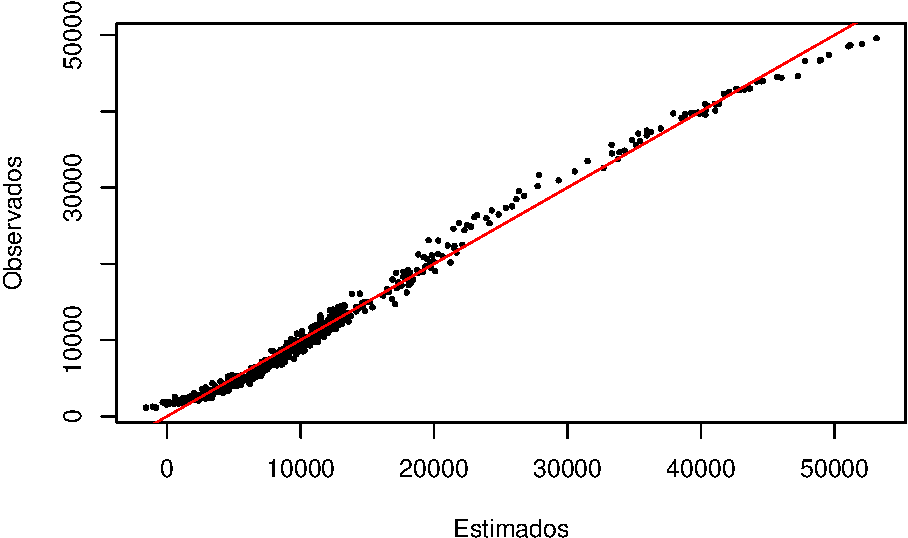
\includegraphics[keepaspectratio]{index_files/figure-latex/unnamed-chunk-22-1.pdf}}

\begin{Shaded}
\begin{Highlighting}[]
\FunctionTok{plot}\NormalTok{(}
\NormalTok{  modelo\_completo}\SpecialCharTok{$}\NormalTok{fitted.values,}
\NormalTok{  modelo\_completo}\SpecialCharTok{$}\NormalTok{residuals, }
  \AttributeTok{xlab =}\StringTok{"estimados"}\NormalTok{,}
  \AttributeTok{ylab=}\StringTok{"residuos"}\NormalTok{,}
  \AttributeTok{pch=}\DecValTok{20}\NormalTok{,}
  \AttributeTok{cex=}\FloatTok{0.5}
\NormalTok{)}
\FunctionTok{abline}\NormalTok{(}\AttributeTok{h=}\DecValTok{0}\NormalTok{,}\AttributeTok{col=}\StringTok{"red"}\NormalTok{)}
\end{Highlighting}
\end{Shaded}

\pandocbounded{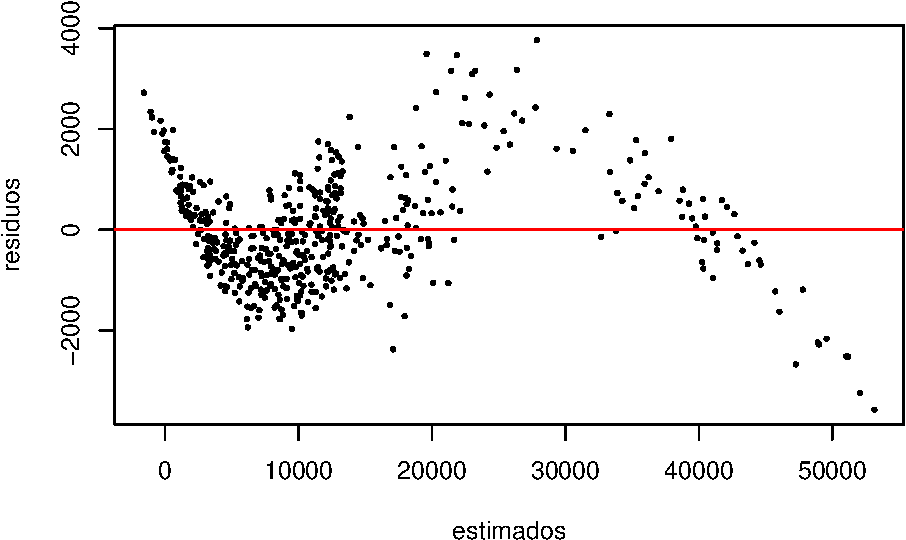
\includegraphics[keepaspectratio]{index_files/figure-latex/unnamed-chunk-23-1.pdf}}

\paragraph{Tests}\label{tests}

\textbf{Prueba de homocedasticidad}

\begin{Shaded}
\begin{Highlighting}[]
\FunctionTok{ncvTest}\NormalTok{(modelo\_completo)}
\end{Highlighting}
\end{Shaded}

\begin{verbatim}
## 
## 
## 
## data:  
## = 351173941, p-value < 2.2e-16
\end{verbatim}

En base al p-valor menor a 0.05, se tiene suficiente evidencia de que la
\textbf{varianza de los residuos no es constante}, es decir, no se
cumple la homocedasticidad.

\textbf{Prueba de normalidad de los errores}

\begin{Shaded}
\begin{Highlighting}[]
\NormalTok{qq\_completo }\OtherTok{\textless{}{-}} \FunctionTok{qqnorm}\NormalTok{(modelo\_completo}\SpecialCharTok{$}\NormalTok{residuals)}
\FunctionTok{qqline}\NormalTok{(modelo\_completo}\SpecialCharTok{$}\NormalTok{residuals)}
\end{Highlighting}
\end{Shaded}

\pandocbounded{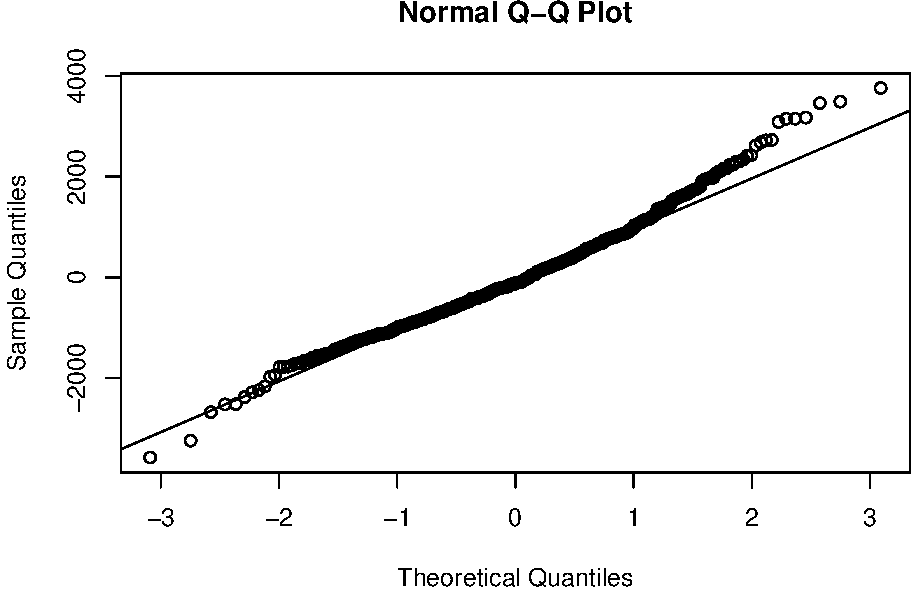
\includegraphics[keepaspectratio]{index_files/figure-latex/unnamed-chunk-25-1.pdf}}

\begin{Shaded}
\begin{Highlighting}[]
\FunctionTok{shapiro.test}\NormalTok{(modelo\_completo}\SpecialCharTok{$}\NormalTok{residuals)}
\end{Highlighting}
\end{Shaded}

\begin{verbatim}
## 
##  Shapiro-Wilk normality test
## 
## data:  modelo_completo$residuals
## W = 0.98331, p-value = 1.677e-05
\end{verbatim}

En base al p-valor menor a 0.05, contamos con suficiente evidencia para
afirmar que los \textbf{residuos no siguen una distribución normal}.

\begin{Shaded}
\begin{Highlighting}[]
\FunctionTok{shapiro.test}\NormalTok{(}\FunctionTok{rstandard}\NormalTok{(modelo\_completo))}
\end{Highlighting}
\end{Shaded}

\begin{verbatim}
## 
##  Shapiro-Wilk normality test
## 
## data:  rstandard(modelo_completo)
## W = 0.98249, p-value = 1.01e-05
\end{verbatim}

Al ejecutar el test para los residuos estandarizados, se llega a la
misma conclusión respecto a la normalidad de los residuos.

Como se ha fallado en ambos tests, no estamos en condición formal de
aplicar ANOVA. Sin embargo, inspeccionemos su resultado de todas
maneras, según la tabla de análisis de la varianza.

\begin{Shaded}
\begin{Highlighting}[]
\FunctionTok{anova}\NormalTok{(modelo\_completo)}
\end{Highlighting}
\end{Shaded}

\begin{verbatim}
## Analysis of Variance Table
## 
## Response: charges
##                                  Df     Sum Sq    Mean Sq  F value    Pr(>F)    
## sex                               1 5.6614e+08 5.6614e+08   474.88 < 2.2e-16 ***
## smoker                            1 3.9087e+10 3.9087e+10 32786.75 < 2.2e-16 ***
## age                               1 7.7570e+09 7.7570e+09  6506.60 < 2.2e-16 ***
## bmi                               1 1.6345e+09 1.6345e+09  1371.07 < 2.2e-16 ***
## Claim_Amount                      1 6.8192e+08 6.8192e+08   572.00 < 2.2e-16 ***
## past_consultations                1 1.3044e+09 1.3044e+09  1094.15 < 2.2e-16 ***
## num_of_steps                      1 6.3277e+09 6.3277e+09  5307.70 < 2.2e-16 ***
## Number_of_past_hospitalizations   1 6.6481e+08 6.6481e+08   557.65 < 2.2e-16 ***
## Anual_Salary                      1 6.1018e+09 6.1018e+09  5118.27 < 2.2e-16 ***
## Residuals                       490 5.8416e+08 1.1922e+06                       
## ---
## Signif. codes:  0 '***' 0.001 '**' 0.01 '*' 0.05 '.' 0.1 ' ' 1
\end{verbatim}

\begin{Shaded}
\begin{Highlighting}[]
\FunctionTok{extraer\_estadistica\_f}\NormalTok{(modelo\_completo)}
\end{Highlighting}
\end{Shaded}

\begin{verbatim}
##    value 
## 5976.563
\end{verbatim}

\begin{Shaded}
\begin{Highlighting}[]
\FunctionTok{obtener\_p\_valor\_de\_estadistica\_f}\NormalTok{(modelo\_completo)}
\end{Highlighting}
\end{Shaded}

\begin{verbatim}
## value 
##     0
\end{verbatim}

Como el p-valor es mucho menor que 0.05, concluimos que este modelo
tiene sentido. En particular, existe alguna covariable que explica
significativamente la varianza asociada a \texttt{charges}.

\begin{Shaded}
\begin{Highlighting}[]
\FunctionTok{extraer\_info\_t\_student}\NormalTok{(modelo\_completo)}
\end{Highlighting}
\end{Shaded}

\begin{verbatim}
##                                     t value      Pr(>|t|) es_significativo
## sexmale                          1.02617973  3.053132e-01            FALSE
## smokeryes                        1.53299676  1.259220e-01            FALSE
## age                             -5.09735180  4.927953e-07             TRUE
## bmi                             -1.84969716  6.495914e-02            FALSE
## Claim_Amount                     0.63850065  5.234461e-01            FALSE
## past_consultations               0.09390782  9.252208e-01            FALSE
## num_of_steps                    40.43404893 3.256649e-158             TRUE
## Number_of_past_hospitalizations -5.24178980  2.368235e-07             TRUE
## Anual_Salary                    71.54209305 1.626762e-261             TRUE
\end{verbatim}

Por otro lado, según este otro test, solo se puede afirmar para las
variables \texttt{age}, \texttt{num\_of\_steps},
\texttt{Number\_of\_past\_hospitalizations} y \texttt{Anual\_Salary} que
tienen sentido en el modelo.

\paragraph{Puntos aberrantes}\label{puntos-aberrantes}

\begin{Shaded}
\begin{Highlighting}[]
\NormalTok{modelo\_completo.cd }\OtherTok{\textless{}{-}} \FunctionTok{cooks.distance}\NormalTok{(modelo\_completo)}
\NormalTok{modelo\_completo.mcd }\OtherTok{\textless{}{-}} \FunctionTok{mean}\NormalTok{(modelo\_completo.cd)}
\end{Highlighting}
\end{Shaded}

\textbf{Puntos más lejos de 3 promedios}

\begin{Shaded}
\begin{Highlighting}[]
\NormalTok{modelo\_completo.cooked\_1 }\OtherTok{\textless{}{-}} \FunctionTok{which}\NormalTok{(modelo\_completo.cd }\SpecialCharTok{\textgreater{}} \DecValTok{3}\SpecialCharTok{*}\NormalTok{modelo\_completo.mcd)}
\NormalTok{modelo\_completo.cooked\_1}
\end{Highlighting}
\end{Shaded}

\begin{verbatim}
##   2  11  14  19  29  31  68  78  85 106 129 138 162 168 223 225 240 242 258 260 267 292 299 316 329 331 347 362 365 373 385 396 412 449 453 455 486 496 
##   2  11  14  19  29  31  68  78  85 106 129 138 162 168 223 225 240 242 258 260 267 292 299 316 329 331 347 362 365 373 385 396 412 449 453 455 486 496
\end{verbatim}

Según aquel criterio, se tienen 38 puntos aberrantes \ldots{} una
cantidad significativa.

\textbf{Puntos más lejos de cuatro veces los regresores}

\begin{Shaded}
\begin{Highlighting}[]
\NormalTok{modelo\_completo.cooked\_2 }\OtherTok{\textless{}{-}} \FunctionTok{which}\NormalTok{(modelo\_completo.cd }\SpecialCharTok{\textgreater{}}\NormalTok{ (}\DecValTok{4} \SpecialCharTok{/} \FunctionTok{dim}\NormalTok{(obs)))}
\NormalTok{modelo\_completo.cooked\_2}
\end{Highlighting}
\end{Shaded}

\begin{verbatim}
##  11  19  29  31  85 129 223 225 263 267 299 329 331 347 365 373 385 449 453 455 
##  11  19  29  31  85 129 223 225 263 267 299 329 331 347 365 373 385 449 453 455
\end{verbatim}

Según este otro criterio, se tienen 20 puntos aberrantes, también una
cantidad significativa.

\textbf{Mayores apalancamientos}: Resaltamos en rojo los 10 puntos con
mayor apalancamiento.

\begin{Shaded}
\begin{Highlighting}[]
\NormalTok{modelo\_completo.graficos\_apalancamiento }\OtherTok{\textless{}{-}} \FunctionTok{resaltar\_n\_puntos\_con\_mayor\_apalancamiento}\NormalTok{(modelo\_completo, }\DecValTok{10}\NormalTok{)}

\NormalTok{modelo\_completo.graficos\_apalancamiento}\SpecialCharTok{$}\FunctionTok{est\_vs\_obs}\NormalTok{()}
\end{Highlighting}
\end{Shaded}

\pandocbounded{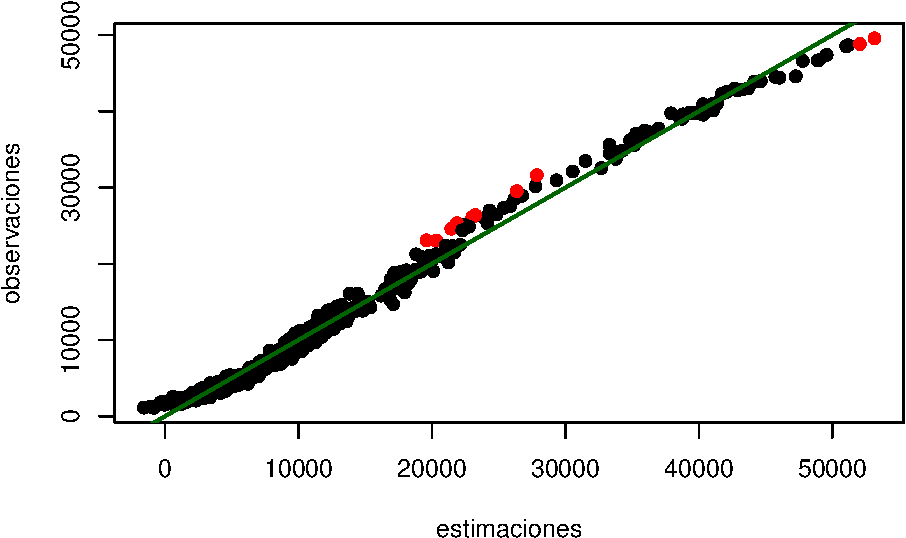
\includegraphics[keepaspectratio]{index_files/figure-latex/unnamed-chunk-33-1.pdf}}

\begin{Shaded}
\begin{Highlighting}[]
\NormalTok{modelo\_completo.graficos\_apalancamiento}\SpecialCharTok{$}\FunctionTok{est\_vs\_res}\NormalTok{()}
\end{Highlighting}
\end{Shaded}

\pandocbounded{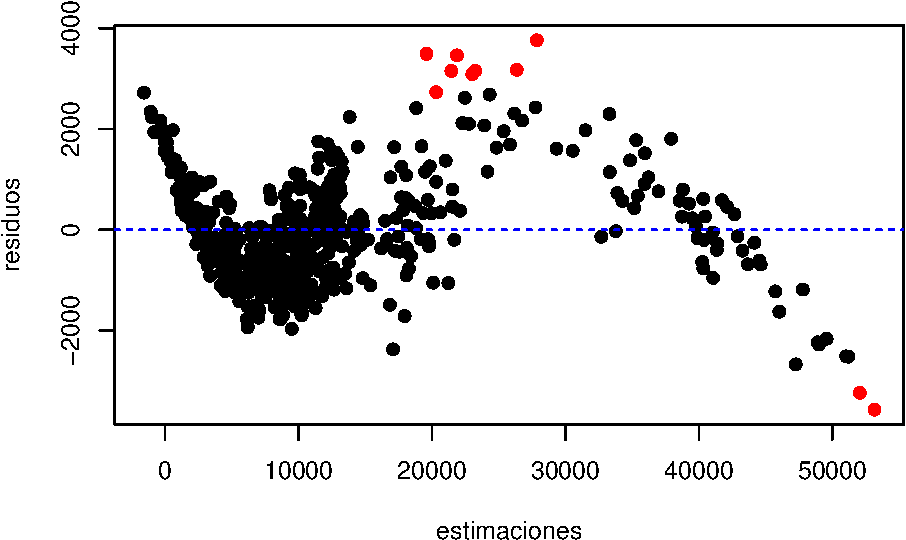
\includegraphics[keepaspectratio]{index_files/figure-latex/unnamed-chunk-33-2.pdf}}

\subsubsection{Modelo tras remover puntos
aberrantes}\label{modelo-tras-remover-puntos-aberrantes}

\begin{Shaded}
\begin{Highlighting}[]
\NormalTok{obs\_sin\_aber }\OtherTok{\textless{}{-}}\NormalTok{ obs[}\SpecialCharTok{{-}}\NormalTok{modelo\_completo.cooked\_1,]}
\NormalTok{obs\_sin\_aber}
\end{Highlighting}
\end{Shaded}

\begin{verbatim}
## # A tibble: 462 x 10
##    sex    smoker   age   bmi Claim_Amount past_consultations num_of_steps Number_of_past_hospitalizations Anual_Salary charges
##    <chr>  <chr>  <dbl> <dbl>        <dbl>              <dbl>        <dbl>                           <dbl>        <dbl>   <dbl>
##  1 male   no        28  33.8       24108.                 18       983349                               1   481649496.  19673.
##  2 male   yes       33  27.1       39953.                 27       996320                               1   453727467.  19041.
##  3 female no        48  28.9       45756.                 24       912509                               1   178469706.   9249.
##  4 male   no        63  31.4       34046.                 14       953355                               1   233696716.  13974.
##  5 male   no        48  34.3       36944.                 18       926940                               1   101378109.   9563.
##  6 female no        59  32.4       44302.                 18       940460                               1   289788380.  14591.
##  7 male   no        38  34.7        8821.                 12       880463                               1    85599131.   6082.
##  8 female no        63  31.8       26904.                 11       954102                               1   194691807.  13881.
##  9 female no        22  24.3        5289.                  8       764144                               0    83114999.   2150.
## 10 female no        54  31.9       41178.                 24       919493                               1   149223188.  10929.
## # i 452 more rows
\end{verbatim}

\begin{Shaded}
\begin{Highlighting}[]
\NormalTok{mod\_com\_2 }\OtherTok{\textless{}{-}} \FunctionTok{lm}\NormalTok{(charges }\SpecialCharTok{\textasciitilde{}}\NormalTok{ ., obs\_sin\_aber)}
\FunctionTok{sum.lm}\NormalTok{(mod\_com\_2)}
\end{Highlighting}
\end{Shaded}

\begin{verbatim}
## 
## Call:
## lm(formula = charges ~ ., data = obs_sin_aber)
## 
## Residuals:
##      Min       1Q   Median       3Q      Max 
## -2250.13  -580.13   -19.38   534.20  2564.82 
## 
## Coefficients:
##                                                 2.5 %     97.5 % Std. Error t value Pr(>|t|)    
## (Intercept)                     -4.026e+04 -4.196e+04 -3.857e+04  8.628e+02 -46.665  < 2e-16 ***
## sexmale                         -3.150e+01 -1.801e+02  1.172e+02  7.564e+01  -0.416 0.677332    
## smokeryes                        8.137e+02  3.846e+02  1.243e+03  2.183e+02   3.726 0.000219 ***
## age                             -1.011e+01 -1.887e+01 -1.348e+00  4.457e+00  -2.268 0.023820 *  
## bmi                             -9.743e+00 -2.315e+01  3.664e+00  6.823e+00  -1.428 0.153950    
## Claim_Amount                    -1.612e-03 -6.884e-03  3.660e-03  2.683e-03  -0.601 0.548244    
## past_consultations               4.894e+00 -7.653e+00  1.744e+01  6.384e+00   0.767 0.443772    
## num_of_steps                     5.521e-02  5.288e-02  5.754e-02  1.185e-03  46.586  < 2e-16 ***
## Number_of_past_hospitalizations -1.900e+03 -2.209e+03 -1.591e+03  1.574e+02 -12.075  < 2e-16 ***
## Anual_Salary                     1.546e-05  1.510e-05  1.581e-05  1.817e-07  85.090  < 2e-16 ***
## ---
## Signif. codes:  0 '***' 0.001 '**' 0.01 '*' 0.05 '.' 0.1 ' ' 1
## 
## Residual standard error: 795.8 on 452 degrees of freedom
## Multiple R-squared:  0.994,  Adjusted R-squared:  0.9939 
## F-statistic:  8345 on 9 and 452 DF,  p-value: < 2.2e-16
\end{verbatim}

Note que el porcentaje de varianza explicada aumentó de 99.1\% a
\textbf{99.4\%}.

\begin{Shaded}
\begin{Highlighting}[]
\FunctionTok{calcular\_rse}\NormalTok{(modelo\_completo)}
\end{Highlighting}
\end{Shaded}

\begin{verbatim}
## [1] 1091.864
\end{verbatim}

\begin{Shaded}
\begin{Highlighting}[]
\FunctionTok{calcular\_rse}\NormalTok{(mod\_com\_2)}
\end{Highlighting}
\end{Shaded}

\begin{verbatim}
## [1] 795.7768
\end{verbatim}

Asimismo, resaltamos que el \textbf{residuo promedio es menor} en el
modelo tras remover puntos aberrantes.

\begin{Shaded}
\begin{Highlighting}[]
\FunctionTok{plot}\NormalTok{(}
\NormalTok{  mod\_com\_2}\SpecialCharTok{$}\NormalTok{fitted.values,}
\NormalTok{  obs\_sin\_aber}\SpecialCharTok{$}\NormalTok{charges,}
  \AttributeTok{xlab =}\StringTok{"Estimados"}\NormalTok{,}
  \AttributeTok{ylab=}\StringTok{"Observados"}\NormalTok{,}
  \AttributeTok{pch=}\DecValTok{20}\NormalTok{,}
  \AttributeTok{cex=}\FloatTok{0.5}
\NormalTok{)}
\FunctionTok{abline}\NormalTok{(}\DecValTok{0}\NormalTok{,}\DecValTok{1}\NormalTok{,}\AttributeTok{col=}\StringTok{"red"}\NormalTok{)}
\end{Highlighting}
\end{Shaded}

\pandocbounded{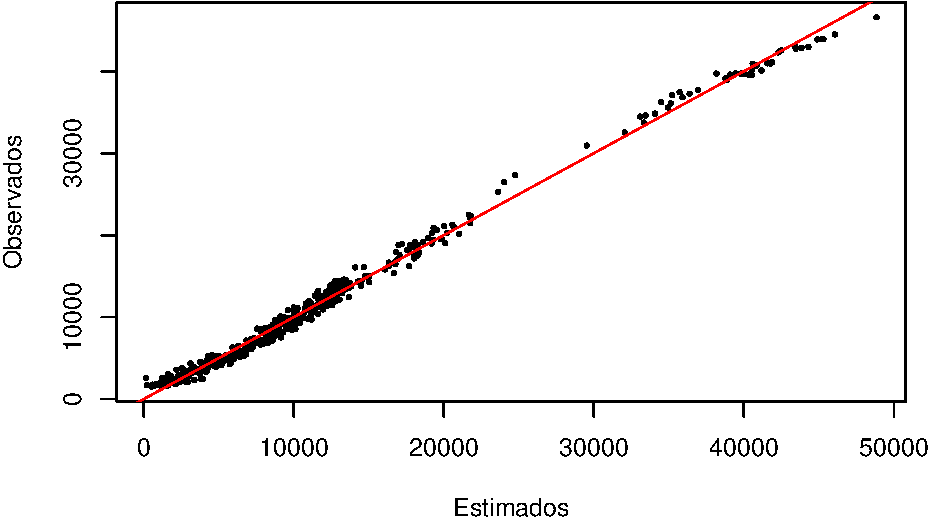
\includegraphics[keepaspectratio]{index_files/figure-latex/unnamed-chunk-37-1.pdf}}

\begin{Shaded}
\begin{Highlighting}[]
\FunctionTok{plot}\NormalTok{(}
\NormalTok{  mod\_com\_2}\SpecialCharTok{$}\NormalTok{fitted.values,}
\NormalTok{  mod\_com\_2}\SpecialCharTok{$}\NormalTok{residuals, }
  \AttributeTok{xlab =}\StringTok{"estimados"}\NormalTok{,}
  \AttributeTok{ylab=}\StringTok{"residuos"}\NormalTok{,}
  \AttributeTok{pch=}\DecValTok{20}\NormalTok{,}
  \AttributeTok{cex=}\FloatTok{0.5}
\NormalTok{)}
\FunctionTok{abline}\NormalTok{(}\AttributeTok{h=}\DecValTok{0}\NormalTok{,}\AttributeTok{col=}\StringTok{"red"}\NormalTok{)}
\end{Highlighting}
\end{Shaded}

\pandocbounded{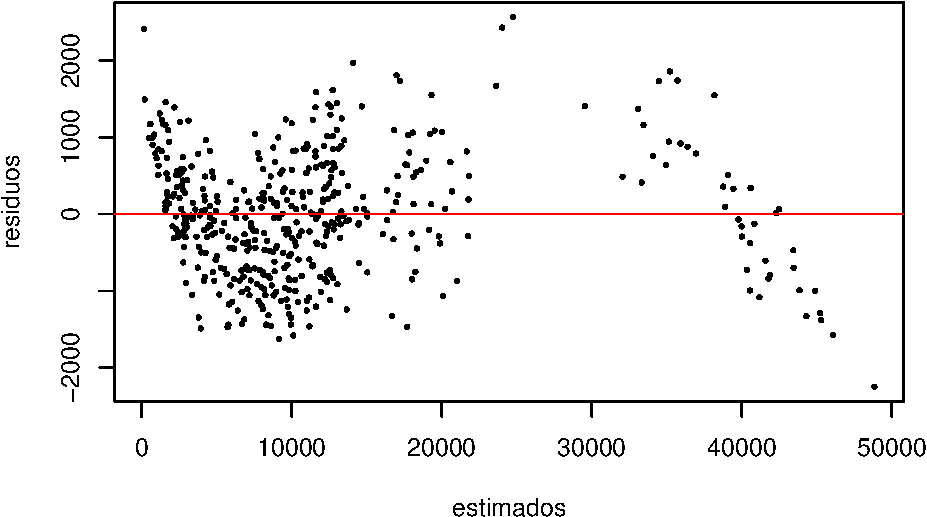
\includegraphics[keepaspectratio]{index_files/figure-latex/unnamed-chunk-38-1.pdf}}

\begin{Shaded}
\begin{Highlighting}[]
\FunctionTok{ncvTest}\NormalTok{(mod\_com\_2)}
\end{Highlighting}
\end{Shaded}

\begin{verbatim}
## 
## 
## 
## data:  
## = 167742048, p-value < 2.2e-16
\end{verbatim}

El p-valor asociado al test de homocedasticidad prácticamente no ha
cambiado.

\begin{Shaded}
\begin{Highlighting}[]
\NormalTok{qq\_completo\_2 }\OtherTok{\textless{}{-}} \FunctionTok{qqnorm}\NormalTok{(mod\_com\_2}\SpecialCharTok{$}\NormalTok{residuals)}
\FunctionTok{qqline}\NormalTok{(mod\_com\_2}\SpecialCharTok{$}\NormalTok{residuals)}
\end{Highlighting}
\end{Shaded}

\pandocbounded{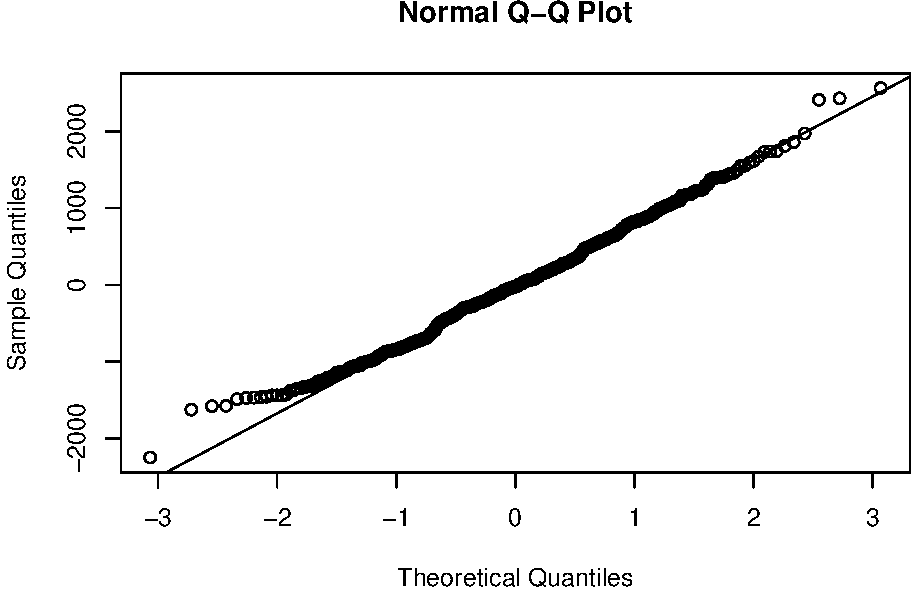
\includegraphics[keepaspectratio]{index_files/figure-latex/unnamed-chunk-40-1.pdf}}

\begin{Shaded}
\begin{Highlighting}[]
\FunctionTok{shapiro.test}\NormalTok{(mod\_com\_2}\SpecialCharTok{$}\NormalTok{residuals)}
\end{Highlighting}
\end{Shaded}

\begin{verbatim}
## 
##  Shapiro-Wilk normality test
## 
## data:  mod_com_2$residuals
## W = 0.99316, p-value = 0.03396
\end{verbatim}

\begin{Shaded}
\begin{Highlighting}[]
\FunctionTok{shapiro.test}\NormalTok{(}\FunctionTok{rstandard}\NormalTok{(mod\_com\_2))}
\end{Highlighting}
\end{Shaded}

\begin{verbatim}
## 
##  Shapiro-Wilk normality test
## 
## data:  rstandard(mod_com_2)
## W = 0.9933, p-value = 0.0379
\end{verbatim}

Por otro lado, el p-valor asociado al Test de Shapiro \textbf{aumentó
significativamente}, de \(1.01*10^{-5}\) a \(0.0379\). Este último valor
es cercano a 0.05, aunque aún menor, por lo cual se sigue evidenciando
la \textbf{no normalidad} de los residuos tras haber removido aquellos
puntos aberrantes.

En base a estas comparaciones, el modelo tras haber removido los puntos
aberrantes resulta \textbf{mejor} que el modelo inicialmente construido.

\subsubsection{Selección reducida de
covariables}\label{selecciuxf3n-reducida-de-covariables}

Calculamos las correlaciones parciales para estas observaciones.

\begin{Shaded}
\begin{Highlighting}[]
\NormalTok{covariables\_numericas}\FloatTok{.2} \OtherTok{\textless{}{-}} \FunctionTok{c}\NormalTok{(}
  \StringTok{"age"}\NormalTok{,}
  \StringTok{"bmi"}\NormalTok{,}
  \StringTok{"Claim\_Amount"}\NormalTok{,}
  \StringTok{"past\_consultations"}\NormalTok{,}
  \StringTok{"num\_of\_steps"}\NormalTok{,}
  \StringTok{"Number\_of\_past\_hospitalizations"}\NormalTok{,}
  \StringTok{"Anual\_Salary"}
\NormalTok{)}

\NormalTok{d.cor}\FloatTok{.2} \OtherTok{\textless{}{-}} \FunctionTok{cor}\NormalTok{(obs\_sin\_aber[, covariables\_numericas}\FloatTok{.2}\NormalTok{])}
\NormalTok{d.inv}\FloatTok{.2} \OtherTok{\textless{}{-}} \FunctionTok{solve}\NormalTok{(d.cor}\FloatTok{.2}\NormalTok{)}

\NormalTok{d.corm}\FloatTok{.2} \OtherTok{\textless{}{-}} \FunctionTok{sqrt}\NormalTok{(}\DecValTok{1{-}1}\SpecialCharTok{/}\FunctionTok{diag}\NormalTok{(d.inv}\FloatTok{.2}\NormalTok{))}
\NormalTok{pd}\FloatTok{.2} \OtherTok{\textless{}{-}} \FunctionTok{length}\NormalTok{(d.corm}\FloatTok{.2}\NormalTok{)  }


\NormalTok{d.part}\FloatTok{.2} \OtherTok{\textless{}{-}}\NormalTok{ d.inv}\FloatTok{.2}
\ControlFlowTok{for}\NormalTok{ (i }\ControlFlowTok{in} \DecValTok{1}\SpecialCharTok{:}\NormalTok{pd}\FloatTok{.2}\NormalTok{) \{}
  \ControlFlowTok{for}\NormalTok{ (j }\ControlFlowTok{in} \DecValTok{1}\SpecialCharTok{:}\NormalTok{(i}\DecValTok{{-}1}\NormalTok{)) \{}
\NormalTok{    d.part}\FloatTok{.2}\NormalTok{[i,j] }\OtherTok{\textless{}{-}} \SpecialCharTok{{-}}\NormalTok{d.inv}\FloatTok{.2}\NormalTok{[i,j]}\SpecialCharTok{/}\FunctionTok{sqrt}\NormalTok{(d.inv}\FloatTok{.2}\NormalTok{[i,i]}\SpecialCharTok{*}\NormalTok{d.inv}\FloatTok{.2}\NormalTok{[j,j])}
\NormalTok{  \}}
\NormalTok{  d.part}\FloatTok{.2}\NormalTok{[i,i] }\OtherTok{\textless{}{-}}\NormalTok{ d.corm}\FloatTok{.2}\NormalTok{[i]}
\NormalTok{  d.part}\FloatTok{.2}\NormalTok{[}\DecValTok{1}\SpecialCharTok{:}\NormalTok{(i}\DecValTok{{-}1}\NormalTok{),i] }\OtherTok{\textless{}{-}}\NormalTok{ d.part}\FloatTok{.2}\NormalTok{[i,}\DecValTok{1}\SpecialCharTok{:}\NormalTok{(i}\DecValTok{{-}1}\NormalTok{)]  }
\NormalTok{\}}
\NormalTok{d.part}\FloatTok{.2}
\end{Highlighting}
\end{Shaded}

\begin{verbatim}
##                                          age         bmi Claim_Amount past_consultations num_of_steps Number_of_past_hospitalizations Anual_Salary
## age                              0.665243871  0.16416635  -0.07721888         0.01344827    0.5839928                     0.006854609   -0.4611240
## bmi                              0.164166348  0.28642055  -0.04976349         0.03776371   -0.1106683                     0.062875288    0.1575645
## Claim_Amount                    -0.077218876 -0.04976349   0.39336416         0.02053137    0.0630846                     0.078407497    0.1021865
## past_consultations               0.013448272  0.03776371   0.02053137         0.54647920    0.1470056                    -0.039271754    0.2168628
## num_of_steps                     0.583992833 -0.11066826   0.06308460         0.14700565    0.8882175                     0.419051171    0.4624652
## Number_of_past_hospitalizations  0.006854609  0.06287529   0.07840750        -0.03927175    0.4190512                     0.834430684    0.3550532
## Anual_Salary                    -0.461124002  0.15756448   0.10218653         0.21686281    0.4624652                     0.355053223    0.8544968
\end{verbatim}

\begin{Shaded}
\begin{Highlighting}[]
\NormalTok{vals\_diag}\FloatTok{.2} \OtherTok{\textless{}{-}} \FunctionTok{diag}\NormalTok{(d.part}\FloatTok{.2}\NormalTok{)}
\NormalTok{max\_col\_indices}\FloatTok{.2} \OtherTok{\textless{}{-}} \FunctionTok{apply}\NormalTok{(d.part}\FloatTok{.2}\NormalTok{, }\DecValTok{1}\NormalTok{, which.max)}
\NormalTok{idx\_ordenados}\FloatTok{.2} \OtherTok{\textless{}{-}} \FunctionTok{order}\NormalTok{(vals\_diag}\FloatTok{.2}\NormalTok{, }\AttributeTok{decreasing =} \ConstantTok{TRUE}\NormalTok{)}
\NormalTok{ordenados\_vals\_diag}\FloatTok{.2} \OtherTok{\textless{}{-}}\NormalTok{ vals\_diag}\FloatTok{.2}\NormalTok{[idx\_ordenados}\FloatTok{.2}\NormalTok{]}

\FunctionTok{data.frame}\NormalTok{(}\AttributeTok{correlacion\_parcial =}\NormalTok{ ordenados\_vals\_diag}\FloatTok{.2}\NormalTok{)}
\end{Highlighting}
\end{Shaded}

\begin{verbatim}
##                                 correlacion_parcial
## num_of_steps                              0.8882175
## Anual_Salary                              0.8544968
## Number_of_past_hospitalizations           0.8344307
## age                                       0.6652439
## past_consultations                        0.5464792
## Claim_Amount                              0.3933642
## bmi                                       0.2864205
\end{verbatim}

Note que aún existen covariables con correlación parcial elevada
(\texttt{num\_of\_steps}, \texttt{Anual\_Salary} y
\texttt{Number\_of\_past\_hospitalizations}), mayor que 0.8; pero ya no
existe covariable con correlación parcial mayor a \(0.9\).

\pandocbounded{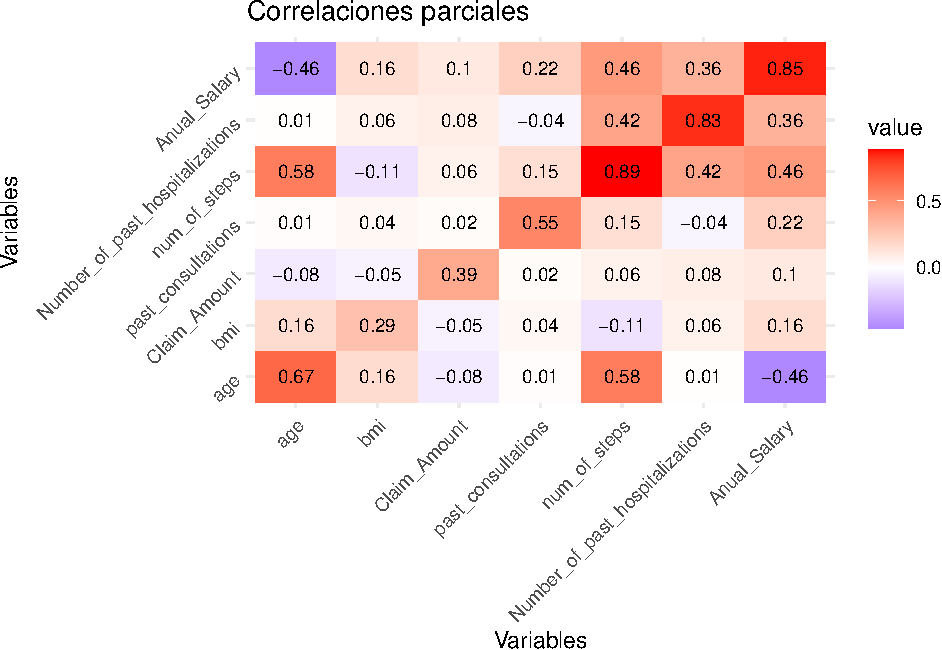
\includegraphics[keepaspectratio]{index_files/figure-latex/unnamed-chunk-42-1.pdf}}

Sin embargo, los valores pequeños en valor absoluto para correlación
parcial entre par de covariables implica que existe \textbf{poca
multicolinealidad} entre las covariables.

\begin{Shaded}
\begin{Highlighting}[]
\NormalTok{modelo\_nulo }\OtherTok{\textless{}{-}} \FunctionTok{lm}\NormalTok{(charges }\SpecialCharTok{\textasciitilde{}} \DecValTok{1}\NormalTok{, obs\_sin\_aber)}
\NormalTok{modelo\_completo}\FloatTok{.2} \OtherTok{\textless{}{-}} \FunctionTok{lm}\NormalTok{(charges }\SpecialCharTok{\textasciitilde{}}\NormalTok{ ., obs\_sin\_aber)}
\end{Highlighting}
\end{Shaded}

\begin{Shaded}
\begin{Highlighting}[]
\NormalTok{modelo\_forward }\OtherTok{\textless{}{-}} \FunctionTok{step}\NormalTok{(}
\NormalTok{  modelo\_nulo,}
  \AttributeTok{scope =} \FunctionTok{list}\NormalTok{(}
    \AttributeTok{lower =}\NormalTok{ modelo\_nulo,}
    \AttributeTok{upper =}\NormalTok{ modelo\_completo}\FloatTok{.2}
\NormalTok{  ),}
  \AttributeTok{direction =} \StringTok{"forward"}\NormalTok{,}
  \AttributeTok{trace =} \DecValTok{0}
\NormalTok{)}

\NormalTok{modelo\_backward }\OtherTok{\textless{}{-}} \FunctionTok{step}\NormalTok{(}
\NormalTok{  modelo\_completo}\FloatTok{.2}\NormalTok{,}
  \AttributeTok{scope =} \FunctionTok{list}\NormalTok{(}
    \AttributeTok{lower =}\NormalTok{ modelo\_nulo,}
    \AttributeTok{upper =}\NormalTok{ modelo\_completo}\FloatTok{.2}
\NormalTok{  ),}
  \AttributeTok{direction =} \StringTok{"backward"}\NormalTok{,}
  \AttributeTok{trace =} \DecValTok{0}
\NormalTok{)}

\NormalTok{modelo\_both }\OtherTok{\textless{}{-}} \FunctionTok{step}\NormalTok{(}
\NormalTok{  modelo\_nulo,}
  \AttributeTok{scope =} \FunctionTok{list}\NormalTok{(}
    \AttributeTok{lower =}\NormalTok{ modelo\_nulo,}
    \AttributeTok{upper =}\NormalTok{ modelo\_completo}\FloatTok{.2}
\NormalTok{  ),}
  \AttributeTok{direction =} \StringTok{"both"}\NormalTok{,}
  \AttributeTok{trace =} \DecValTok{0}
\NormalTok{)}
\end{Highlighting}
\end{Shaded}

\begin{Shaded}
\begin{Highlighting}[]
\FunctionTok{sum.lm}\NormalTok{(modelo\_forward)}
\end{Highlighting}
\end{Shaded}

\begin{verbatim}
## 
## Call:
## lm(formula = charges ~ Anual_Salary + num_of_steps + Number_of_past_hospitalizations + 
##     smoker + age + bmi, data = obs_sin_aber)
## 
## Residuals:
##      Min       1Q   Median       3Q      Max 
## -2281.32  -580.54   -16.49   544.60  2573.51 
## 
## Coefficients:
##                                                 2.5 %     97.5 % Std. Error t value Pr(>|t|)    
## (Intercept)                     -4.036e+04 -4.204e+04 -3.868e+04  8.553e+02 -47.182  < 2e-16 ***
## Anual_Salary                     1.547e-05  1.512e-05  1.582e-05  1.774e-07  87.232  < 2e-16 ***
## num_of_steps                     5.532e-02  5.301e-02  5.762e-02  1.173e-03  47.146  < 2e-16 ***
## Number_of_past_hospitalizations -1.909e+03 -2.216e+03 -1.602e+03  1.561e+02 -12.227  < 2e-16 ***
## smokeryes                        8.004e+02  3.744e+02  1.226e+03  2.168e+02   3.692 0.000249 ***
## age                             -1.006e+01 -1.880e+01 -1.334e+00  4.443e+00  -2.265 0.023956 *  
## bmi                             -9.569e+00 -2.292e+01  3.777e+00  6.792e+00  -1.409 0.159512    
## ---
## Signif. codes:  0 '***' 0.001 '**' 0.01 '*' 0.05 '.' 0.1 ' ' 1
## 
## Residual standard error: 794 on 455 degrees of freedom
## Multiple R-squared:  0.994,  Adjusted R-squared:  0.9939 
## F-statistic: 1.257e+04 on 6 and 455 DF,  p-value: < 2.2e-16
\end{verbatim}

\begin{Shaded}
\begin{Highlighting}[]
\FunctionTok{sum.lm}\NormalTok{(modelo\_backward)}
\end{Highlighting}
\end{Shaded}

\begin{verbatim}
## 
## Call:
## lm(formula = charges ~ smoker + age + bmi + num_of_steps + Number_of_past_hospitalizations + 
##     Anual_Salary, data = obs_sin_aber)
## 
## Residuals:
##      Min       1Q   Median       3Q      Max 
## -2281.32  -580.54   -16.49   544.60  2573.51 
## 
## Coefficients:
##                                                 2.5 %     97.5 % Std. Error t value Pr(>|t|)    
## (Intercept)                     -4.036e+04 -4.204e+04 -3.868e+04  8.553e+02 -47.182  < 2e-16 ***
## smokeryes                        8.004e+02  3.744e+02  1.226e+03  2.168e+02   3.692 0.000249 ***
## age                             -1.006e+01 -1.880e+01 -1.334e+00  4.443e+00  -2.265 0.023956 *  
## bmi                             -9.569e+00 -2.292e+01  3.777e+00  6.792e+00  -1.409 0.159512    
## num_of_steps                     5.532e-02  5.301e-02  5.762e-02  1.173e-03  47.146  < 2e-16 ***
## Number_of_past_hospitalizations -1.909e+03 -2.216e+03 -1.602e+03  1.561e+02 -12.227  < 2e-16 ***
## Anual_Salary                     1.547e-05  1.512e-05  1.582e-05  1.774e-07  87.232  < 2e-16 ***
## ---
## Signif. codes:  0 '***' 0.001 '**' 0.01 '*' 0.05 '.' 0.1 ' ' 1
## 
## Residual standard error: 794 on 455 degrees of freedom
## Multiple R-squared:  0.994,  Adjusted R-squared:  0.9939 
## F-statistic: 1.257e+04 on 6 and 455 DF,  p-value: < 2.2e-16
\end{verbatim}

\begin{Shaded}
\begin{Highlighting}[]
\FunctionTok{sum.lm}\NormalTok{(modelo\_both)}
\end{Highlighting}
\end{Shaded}

\begin{verbatim}
## 
## Call:
## lm(formula = charges ~ Anual_Salary + num_of_steps + Number_of_past_hospitalizations + 
##     smoker + age + bmi, data = obs_sin_aber)
## 
## Residuals:
##      Min       1Q   Median       3Q      Max 
## -2281.32  -580.54   -16.49   544.60  2573.51 
## 
## Coefficients:
##                                                 2.5 %     97.5 % Std. Error t value Pr(>|t|)    
## (Intercept)                     -4.036e+04 -4.204e+04 -3.868e+04  8.553e+02 -47.182  < 2e-16 ***
## Anual_Salary                     1.547e-05  1.512e-05  1.582e-05  1.774e-07  87.232  < 2e-16 ***
## num_of_steps                     5.532e-02  5.301e-02  5.762e-02  1.173e-03  47.146  < 2e-16 ***
## Number_of_past_hospitalizations -1.909e+03 -2.216e+03 -1.602e+03  1.561e+02 -12.227  < 2e-16 ***
## smokeryes                        8.004e+02  3.744e+02  1.226e+03  2.168e+02   3.692 0.000249 ***
## age                             -1.006e+01 -1.880e+01 -1.334e+00  4.443e+00  -2.265 0.023956 *  
## bmi                             -9.569e+00 -2.292e+01  3.777e+00  6.792e+00  -1.409 0.159512    
## ---
## Signif. codes:  0 '***' 0.001 '**' 0.01 '*' 0.05 '.' 0.1 ' ' 1
## 
## Residual standard error: 794 on 455 degrees of freedom
## Multiple R-squared:  0.994,  Adjusted R-squared:  0.9939 
## F-statistic: 1.257e+04 on 6 and 455 DF,  p-value: < 2.2e-16
\end{verbatim}

\begin{Shaded}
\begin{Highlighting}[]
\FunctionTok{calcular\_rse}\NormalTok{(modelo\_forward)}
\end{Highlighting}
\end{Shaded}

\begin{verbatim}
## [1] 794.0415
\end{verbatim}

\begin{Shaded}
\begin{Highlighting}[]
\FunctionTok{calcular\_rse}\NormalTok{(modelo\_backward)}
\end{Highlighting}
\end{Shaded}

\begin{verbatim}
## [1] 794.0415
\end{verbatim}

\begin{Shaded}
\begin{Highlighting}[]
\FunctionTok{calcular\_rse}\NormalTok{(modelo\_both)}
\end{Highlighting}
\end{Shaded}

\begin{verbatim}
## [1] 794.0415
\end{verbatim}

\begin{Shaded}
\begin{Highlighting}[]
\FunctionTok{calcular\_rse}\NormalTok{(modelo\_completo)}
\end{Highlighting}
\end{Shaded}

\begin{verbatim}
## [1] 1091.864
\end{verbatim}

\begin{Shaded}
\begin{Highlighting}[]
\FunctionTok{calcular\_rse}\NormalTok{(mod\_com\_2)}
\end{Highlighting}
\end{Shaded}

\begin{verbatim}
## [1] 795.7768
\end{verbatim}

\subsubsection{Modelo final}\label{modelo-final}

Comparando las covariables finales de los tres últimos modelos creados,
además de sus coeficientes respectivos, note que se trata de un único
modelo.

Asimimo, aquel modelo presenta un \(R^2\) elevado, similar al del previo
mejor modelo, también con un valor aproximado a 99.4\%.

No obstante, recalcamos que el nuevo modelo presenta un \textbf{residuo
promedio menor} que el del mejor modelo que habíamos construído hasta
ahora.

En ese sentido, el mejor modelo que planteamos es \texttt{modelo\_both}.
Este presenta como covariables a \texttt{age}, \texttt{Anual\_Salary},
\texttt{bmi}, \texttt{smoker}, \texttt{num\_of\_steps} y
\texttt{Number\_of\_past\_hospitalizations}.

\begin{Shaded}
\begin{Highlighting}[]
\NormalTok{modelo\_both}
\end{Highlighting}
\end{Shaded}

\begin{verbatim}
## 
## Call:
## lm(formula = charges ~ Anual_Salary + num_of_steps + Number_of_past_hospitalizations + 
##     smoker + age + bmi, data = obs_sin_aber)
## 
## Coefficients:
##                     (Intercept)                     Anual_Salary                     num_of_steps  Number_of_past_hospitalizations                        smokeryes                              age  
##                      -4.036e+04                        1.547e-05                        5.532e-02                       -1.909e+03                        8.004e+02                       -1.006e+01  
##                             bmi  
##                      -9.569e+00
\end{verbatim}

\begin{Shaded}
\begin{Highlighting}[]
\FunctionTok{plot}\NormalTok{(}
\NormalTok{  modelo\_both}\SpecialCharTok{$}\NormalTok{fitted.values,}
\NormalTok{  obs\_sin\_aber}\SpecialCharTok{$}\NormalTok{charges,}
  \AttributeTok{xlab =}\StringTok{"Estimados"}\NormalTok{,}
  \AttributeTok{ylab=}\StringTok{"Observados"}\NormalTok{,}
  \AttributeTok{pch=}\DecValTok{20}\NormalTok{,}
  \AttributeTok{cex=}\FloatTok{0.5}
\NormalTok{)}
\FunctionTok{abline}\NormalTok{(}\DecValTok{0}\NormalTok{,}\DecValTok{1}\NormalTok{,}\AttributeTok{col=}\StringTok{"red"}\NormalTok{)}
\end{Highlighting}
\end{Shaded}

\pandocbounded{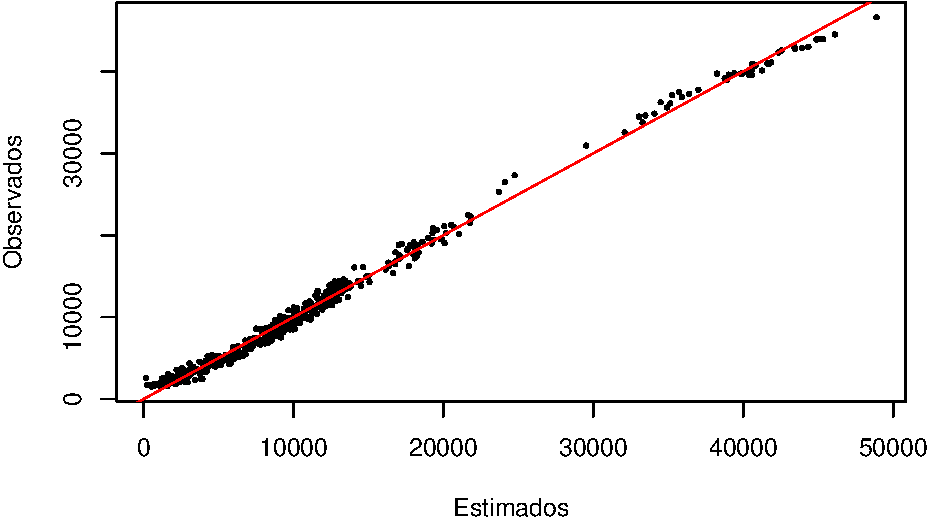
\includegraphics[keepaspectratio]{index_files/figure-latex/unnamed-chunk-48-1.pdf}}

\begin{Shaded}
\begin{Highlighting}[]
\FunctionTok{plot}\NormalTok{(}
\NormalTok{  modelo\_both}\SpecialCharTok{$}\NormalTok{fitted.values,}
\NormalTok{  modelo\_both}\SpecialCharTok{$}\NormalTok{residuals, }
  \AttributeTok{xlab =}\StringTok{"estimados"}\NormalTok{,}
  \AttributeTok{ylab=}\StringTok{"residuos"}\NormalTok{,}
  \AttributeTok{pch=}\DecValTok{20}\NormalTok{,}
  \AttributeTok{cex=}\FloatTok{0.5}
\NormalTok{)}
\FunctionTok{abline}\NormalTok{(}\AttributeTok{h=}\DecValTok{0}\NormalTok{,}\AttributeTok{col=}\StringTok{"red"}\NormalTok{)}
\end{Highlighting}
\end{Shaded}

\pandocbounded{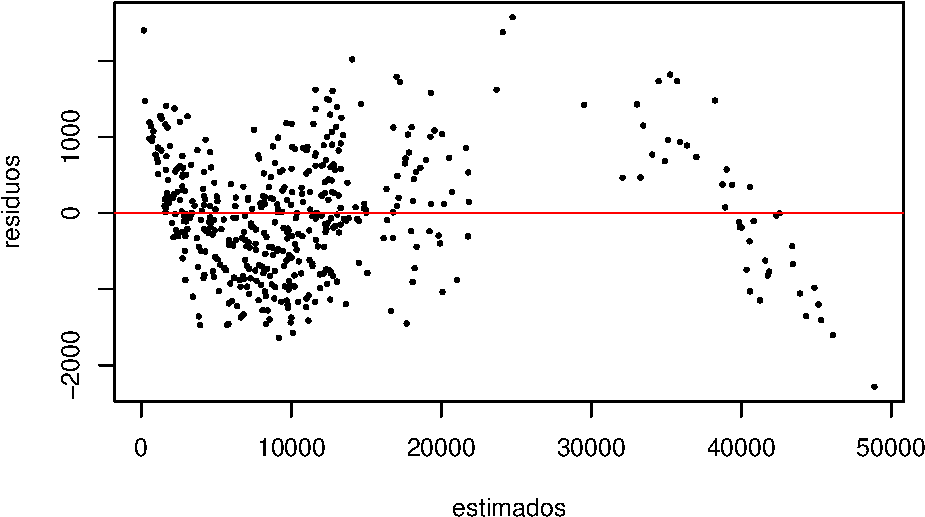
\includegraphics[keepaspectratio]{index_files/figure-latex/unnamed-chunk-49-1.pdf}}

\textbf{Prueba de homocedasticidad}

\begin{Shaded}
\begin{Highlighting}[]
\FunctionTok{ncvTest}\NormalTok{(modelo\_both)}
\end{Highlighting}
\end{Shaded}

\begin{verbatim}
## 
## 
## 
## data:  
## = 167917219, p-value < 2.2e-16
\end{verbatim}

\textbf{Prueba de normalidad de los errores}

\begin{Shaded}
\begin{Highlighting}[]
\NormalTok{qq\_completo\_3 }\OtherTok{\textless{}{-}} \FunctionTok{qqnorm}\NormalTok{(modelo\_both}\SpecialCharTok{$}\NormalTok{residuals)}
\FunctionTok{qqline}\NormalTok{(modelo\_both}\SpecialCharTok{$}\NormalTok{residuals)}
\end{Highlighting}
\end{Shaded}

\pandocbounded{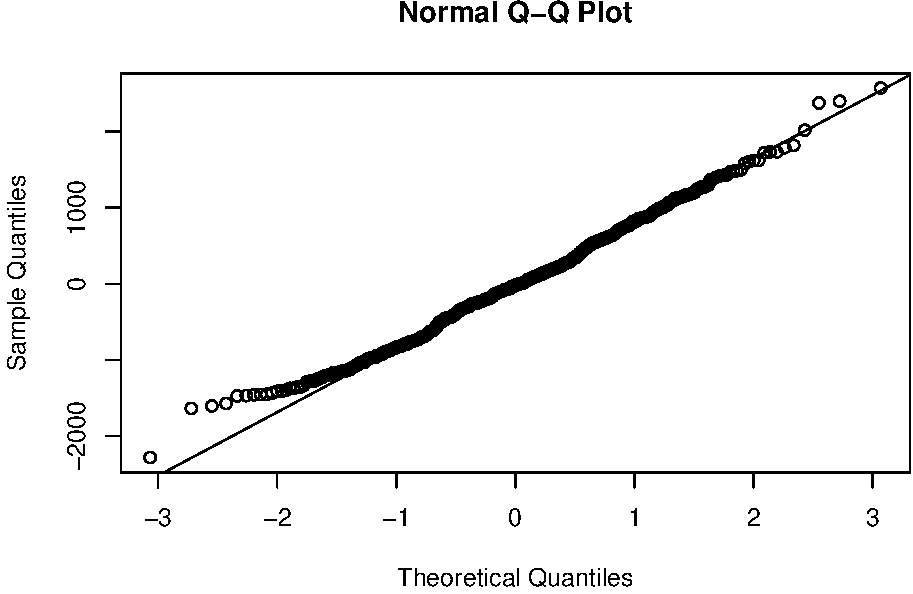
\includegraphics[keepaspectratio]{index_files/figure-latex/unnamed-chunk-51-1.pdf}}

\begin{Shaded}
\begin{Highlighting}[]
\FunctionTok{shapiro.test}\NormalTok{(modelo\_both}\SpecialCharTok{$}\NormalTok{residuals)}
\end{Highlighting}
\end{Shaded}

\begin{verbatim}
## 
##  Shapiro-Wilk normality test
## 
## data:  modelo_both$residuals
## W = 0.99308, p-value = 0.03182
\end{verbatim}

\begin{Shaded}
\begin{Highlighting}[]
\FunctionTok{shapiro.test}\NormalTok{(}\FunctionTok{rstandard}\NormalTok{(modelo\_both))}
\end{Highlighting}
\end{Shaded}

\begin{verbatim}
## 
##  Shapiro-Wilk normality test
## 
## data:  rstandard(modelo_both)
## W = 0.99322, p-value = 0.03554
\end{verbatim}

Para este modelo también se concluye que no se cumple la
homocedasticidad y que los residuos no presentan una distribución
normal.

\begin{Shaded}
\begin{Highlighting}[]
\FunctionTok{anova}\NormalTok{(modelo\_both)}
\end{Highlighting}
\end{Shaded}

\begin{verbatim}
## Analysis of Variance Table
## 
## Response: charges
##                                  Df     Sum Sq    Mean Sq    F value    Pr(>F)    
## Anual_Salary                      1 4.3922e+10 4.3922e+10 69661.4333 < 2.2e-16 ***
## num_of_steps                      1 3.4856e+09 3.4856e+09  5528.3339 < 2.2e-16 ***
## Number_of_past_hospitalizations   1 1.1417e+08 1.1417e+08   181.0800 < 2.2e-16 ***
## smoker                            1 3.1743e+07 3.1743e+07    50.3452 4.973e-12 ***
## age                               1 3.1258e+06 3.1258e+06     4.9577   0.02646 *  
## bmi                               1 1.2518e+06 1.2518e+06     1.9853   0.15951    
## Residuals                       455 2.8688e+08 6.3050e+05                         
## ---
## Signif. codes:  0 '***' 0.001 '**' 0.01 '*' 0.05 '.' 0.1 ' ' 1
\end{verbatim}

\begin{Shaded}
\begin{Highlighting}[]
\FunctionTok{extraer\_estadistica\_f}\NormalTok{(modelo\_both)}
\end{Highlighting}
\end{Shaded}

\begin{verbatim}
##    value 
## 12571.36
\end{verbatim}

\begin{Shaded}
\begin{Highlighting}[]
\FunctionTok{obtener\_p\_valor\_de\_estadistica\_f}\NormalTok{(modelo\_both)}
\end{Highlighting}
\end{Shaded}

\begin{verbatim}
## value 
##     0
\end{verbatim}

\begin{Shaded}
\begin{Highlighting}[]
\FunctionTok{extraer\_info\_t\_student}\NormalTok{(modelo\_both)}
\end{Highlighting}
\end{Shaded}

\begin{verbatim}
##                                    t value      Pr(>|t|) es_significativo
## Anual_Salary                     87.232374 3.440579e-286             TRUE
## num_of_steps                     47.145582 3.122331e-177             TRUE
## Number_of_past_hospitalizations -12.227038  6.354538e-30             TRUE
## smokeryes                         3.692271  2.492338e-04             TRUE
## age                              -2.265428  2.395574e-02             TRUE
## bmi                              -1.409021  1.595120e-01            FALSE
\end{verbatim}

A partir de estos dos últimos tests, se concluye que este modelo tiene
sentido, pero que la covariable \texttt{bmi} no es significativa para
ese modelo.

En base a que residuos de este modelo no satisfacen la hipótesis de
homocedasticidad ni de distribución normal, no presentaremos los
análisis de ANOVA tipo I, II ni III, por tratarse aquellas hipótesis de
condiciones necesarias.

\subsection{Discusión}\label{discusiuxf3n}

\begin{Shaded}
\begin{Highlighting}[]
\FunctionTok{sum.lm}\NormalTok{(modelo\_completo)}
\end{Highlighting}
\end{Shaded}

\begin{verbatim}
## 
## Call:
## lm(formula = charges ~ ., data = obs)
## 
## Residuals:
##     Min      1Q  Median      3Q     Max 
## -3574.8  -728.0  -121.6   631.4  3762.3 
## 
## Coefficients:
##                                                 2.5 %     97.5 % Std. Error t value Pr(>|t|)    
## (Intercept)                     -4.223e+04 -4.430e+04 -4.016e+04  1.055e+03 -40.029  < 2e-16 ***
## sexmale                          1.018e+02 -9.310e+01  2.967e+02  9.919e+01   1.026    0.305    
## smokeryes                        3.807e+02 -1.072e+02  8.686e+02  2.483e+02   1.533    0.126    
## age                             -2.649e+01 -3.670e+01 -1.628e+01  5.196e+00  -5.097 4.93e-07 ***
## bmi                             -1.680e+01 -3.465e+01  1.046e+00  9.083e+00  -1.850    0.065 .  
## Claim_Amount                     2.238e-03 -4.649e-03  9.125e-03  3.505e-03   0.639    0.523    
## past_consultations               7.868e-01 -1.567e+01  1.725e+01  8.378e+00   0.094    0.925    
## num_of_steps                     5.771e-02  5.491e-02  6.051e-02  1.427e-03  40.434  < 2e-16 ***
## Number_of_past_hospitalizations -1.022e+03 -1.405e+03 -6.391e+02  1.950e+02  -5.242 2.37e-07 ***
## Anual_Salary                     1.451e-05  1.411e-05  1.490e-05  2.028e-07  71.542  < 2e-16 ***
## ---
## Signif. codes:  0 '***' 0.001 '**' 0.01 '*' 0.05 '.' 0.1 ' ' 1
## 
## Residual standard error: 1092 on 490 degrees of freedom
## Multiple R-squared:  0.991,  Adjusted R-squared:  0.9908 
## F-statistic:  5977 on 9 and 490 DF,  p-value: < 2.2e-16
\end{verbatim}

\begin{Shaded}
\begin{Highlighting}[]
\FunctionTok{sum.lm}\NormalTok{(mod\_com\_2)}
\end{Highlighting}
\end{Shaded}

\begin{verbatim}
## 
## Call:
## lm(formula = charges ~ ., data = obs_sin_aber)
## 
## Residuals:
##      Min       1Q   Median       3Q      Max 
## -2250.13  -580.13   -19.38   534.20  2564.82 
## 
## Coefficients:
##                                                 2.5 %     97.5 % Std. Error t value Pr(>|t|)    
## (Intercept)                     -4.026e+04 -4.196e+04 -3.857e+04  8.628e+02 -46.665  < 2e-16 ***
## sexmale                         -3.150e+01 -1.801e+02  1.172e+02  7.564e+01  -0.416 0.677332    
## smokeryes                        8.137e+02  3.846e+02  1.243e+03  2.183e+02   3.726 0.000219 ***
## age                             -1.011e+01 -1.887e+01 -1.348e+00  4.457e+00  -2.268 0.023820 *  
## bmi                             -9.743e+00 -2.315e+01  3.664e+00  6.823e+00  -1.428 0.153950    
## Claim_Amount                    -1.612e-03 -6.884e-03  3.660e-03  2.683e-03  -0.601 0.548244    
## past_consultations               4.894e+00 -7.653e+00  1.744e+01  6.384e+00   0.767 0.443772    
## num_of_steps                     5.521e-02  5.288e-02  5.754e-02  1.185e-03  46.586  < 2e-16 ***
## Number_of_past_hospitalizations -1.900e+03 -2.209e+03 -1.591e+03  1.574e+02 -12.075  < 2e-16 ***
## Anual_Salary                     1.546e-05  1.510e-05  1.581e-05  1.817e-07  85.090  < 2e-16 ***
## ---
## Signif. codes:  0 '***' 0.001 '**' 0.01 '*' 0.05 '.' 0.1 ' ' 1
## 
## Residual standard error: 795.8 on 452 degrees of freedom
## Multiple R-squared:  0.994,  Adjusted R-squared:  0.9939 
## F-statistic:  8345 on 9 and 452 DF,  p-value: < 2.2e-16
\end{verbatim}

\begin{Shaded}
\begin{Highlighting}[]
\FunctionTok{sum.lm}\NormalTok{(modelo\_both)}
\end{Highlighting}
\end{Shaded}

\begin{verbatim}
## 
## Call:
## lm(formula = charges ~ Anual_Salary + num_of_steps + Number_of_past_hospitalizations + 
##     smoker + age + bmi, data = obs_sin_aber)
## 
## Residuals:
##      Min       1Q   Median       3Q      Max 
## -2281.32  -580.54   -16.49   544.60  2573.51 
## 
## Coefficients:
##                                                 2.5 %     97.5 % Std. Error t value Pr(>|t|)    
## (Intercept)                     -4.036e+04 -4.204e+04 -3.868e+04  8.553e+02 -47.182  < 2e-16 ***
## Anual_Salary                     1.547e-05  1.512e-05  1.582e-05  1.774e-07  87.232  < 2e-16 ***
## num_of_steps                     5.532e-02  5.301e-02  5.762e-02  1.173e-03  47.146  < 2e-16 ***
## Number_of_past_hospitalizations -1.909e+03 -2.216e+03 -1.602e+03  1.561e+02 -12.227  < 2e-16 ***
## smokeryes                        8.004e+02  3.744e+02  1.226e+03  2.168e+02   3.692 0.000249 ***
## age                             -1.006e+01 -1.880e+01 -1.334e+00  4.443e+00  -2.265 0.023956 *  
## bmi                             -9.569e+00 -2.292e+01  3.777e+00  6.792e+00  -1.409 0.159512    
## ---
## Signif. codes:  0 '***' 0.001 '**' 0.01 '*' 0.05 '.' 0.1 ' ' 1
## 
## Residual standard error: 794 on 455 degrees of freedom
## Multiple R-squared:  0.994,  Adjusted R-squared:  0.9939 
## F-statistic: 1.257e+04 on 6 and 455 DF,  p-value: < 2.2e-16
\end{verbatim}

Note que el último modelo presentado cuenta con el mayor \(R^2\)
ajustado, 99.39\%, entre los modelos expuestos. Este criterio refuerza
su selección como modelo final para este proyecto.

\begin{Shaded}
\begin{Highlighting}[]
\NormalTok{modelo\_both}
\end{Highlighting}
\end{Shaded}

\begin{verbatim}
## 
## Call:
## lm(formula = charges ~ Anual_Salary + num_of_steps + Number_of_past_hospitalizations + 
##     smoker + age + bmi, data = obs_sin_aber)
## 
## Coefficients:
##                     (Intercept)                     Anual_Salary                     num_of_steps  Number_of_past_hospitalizations                        smokeryes                              age  
##                      -4.036e+04                        1.547e-05                        5.532e-02                       -1.909e+03                        8.004e+02                       -1.006e+01  
##                             bmi  
##                      -9.569e+00
\end{verbatim}

Entre lo positivo de este estudio, recalcamos que el modelo final
presenta un alto valor de \(R^2\). Sin embargo, el hecho que para todos
los modelos que creamos se llegó a concluir no homocedasticidad y
residuos con distribución no normal, parece sugerir que el modelo de
regresión lineal posiblemente no sea el adecuado para estos datos.

En todo caso, resulta posible que un modelo lineal generalizado resulte
más apropiado para el uso con estos datos, en particular debido a la no
homocedasticidad encontrada.

Respecto al mejor modelo que presentamos, analicemos la relevancia de
las covariables que consideró para su definición:

\begin{itemize}
\tightlist
\item
  \texttt{age}: Predictor muy relevante con la variable respuesta, pues,
  como se mencionó en una sección previa, sucede que paciente de mayor
  edad suelen requerir más cuidados médicos, su salud está en mayor
  riesgo, por lo que se espera que la aseguradora cubra más el costo de
  un tratamiento médico. En efecto, tal es el caso, pues el coeficiente
  asociado a \texttt{age} en el modelo resulta negativo. Así, a mayor
  edad del paciente, se espera que pague menos (pues la aseguradora
  cubre mayor costo) por un tratamiento médico.
\item
  \texttt{Anual\_Salary}: En el caso de pacientes con alto ingreso
  anual, se espera que sus tratamientos médicos sean también de alto
  costo. Esto implica que la aseguradora cubra una \textbf{menor
  proporción} del costo médico, pues la cobertura ya resulta alta en
  base al precio total del procedimiento. Esta relación se hace evidente
  en el hecho que el coeficiente asociado a \texttt{Annual\_Salary} es
  positivo; es decir, a mayor salario anual, menos costo cubre la
  aseguradora.
\item
  \texttt{bmi}: La relación entre esta covariable y la variable por
  predecir es muy similar la relación de la edad y la variable por
  predecir. Por ello, el análisis el análogo, y, simplemente recalcamos
  que el modelo resalta lo esperado (en base al coeficiente negativo
  asociado a \texttt{bmi}), pues, a mayor índice de masa corporal
  (\texttt{bmi}), la aseguradora cubre más del costo, por lo cual el
  paciente paga menos.
\item
  \texttt{smoker}: En el modelo, esta covariable categórica ha sido
  convertida en 0 y 1; considerando el caso 1 cuando el paciente es
  fumador. En ese sentido, el coeficiente positivo asociado a esta
  covariable indice que, si el paciente es fumador, entonces su precio a
  pagar por tratamiento médico es también mayor, pues la aseguradora
  cubre \textbf{menos} del costo del procedimiento médico.
\item
  \texttt{num\_of\_steps}: Recordemos que esta covariable la
  interpretamos como un indicador del estado de salud del paciente. Es
  decir, un mayor valor de \texttt{num\_of\_steps} representa un mejor
  estado de salud, de actividad física, del paciente. En ese sentido, es
  coherente que aquella covariable presente un coeficiente positivo
  según el modelo. Esto pues, mientras más saludable sea una persona, su
  gasto por procedimiento médico será mayor; es decir, la aseguradora
  cubrirá una \textbf{menor} cantidad del costo del procedimiento.
\item
  \texttt{Number\_of\_past\_hospitalizations}: Esta covariable es
  posiblemente la que más relación se espera tenga con la variable por
  predecir. El coeficiente negativo asociada a esta covariable es
  coherente con el hecho que, a mayor número de hospitalizaciones
  pasadas, se espera que el seguro cubra una mayor parte del costo del
  procedimiento médico, por lo cual el gasto del paciente es
  \textbf{menor} por procedimiento médico.
\end{itemize}

Como no existe una interpretación física, realista, al caso
\texttt{bmi\ =\ 0}, no interpretaremos el intercepto asociado al modelo.

\subsection{Conclusiones}\label{conclusiones}

\begin{enumerate}
\def\labelenumi{\arabic{enumi}.}
\item
  \textbf{Validación de hipótesis sobre correlaciones}: Se confirmaron
  las hipótesis respecto al tipo de correlación (positiva o negativa)
  entre las covariables del modelo final y el precio por pagar por
  procedimiento médico.
\item
  \textbf{Capacidad predictiva del modelo}: El último modelo presentado
  logró explicar el \textbf{99.4\%} de la varianza en el costo para el
  paciente por procedimiento médico, demostrando así una capacidad
  predictiva alta. Este nivel de precisión sugiere que las variables
  seleccionadas capturan efectivamente los factores determinantes en la
  cobertura de seguros médicos.
\item
  \textbf{Variables más influyentes identificadas}: El análisis reveló
  que las variables más significativas para predecir los costos
  cubiertos son: edad (\texttt{age}), salario anual
  (\texttt{Annual\_Salary}), índice de masa corporal (\texttt{bmi}),
  hábito de fumar (\texttt{smoker}), número de pasos
  (\texttt{num\_of\_steps}), y número de hospitalizaciones previas
  (\texttt{Number\_of\_past\_hospitalizations}). Estas variables
  representan factores demográficos, socioeconómicos y de estilo de vida
  que las aseguradoras consideran en sus decisiones de cobertura.
\item
  \textbf{Limitaciones metodológicas detectadas}: A pesar del alto poder
  predictivo, el modelo no satisface supuestos importante para la
  regresión lineal, la homocedasticidad y la normalidad de los residuos.
  Estas limitaciones sugieren que un modelo lineal simple podría no ser
  la aproximación más adecuada para estos datos.
\item
  \textbf{Recomendación de modelos alternativos}: Los hallazgos de
  heterocedasticidad y no normalidad de residuos indican que un
  \textbf{modelo lineal generalizado (GLM)} podría ser más apropiado
  para este tipo de datos. Estos enfoques alternativos podrían
  proporcionar estimaciones más confiables, además de intervalos de
  confianza más precisos.
\item
  \textbf{Necesidad de validación externa}: Aunque el modelo muestra
  alta precisión en los datos analizados, se recomienda validar estos
  resultados con datos de diferentes poblaciones, sistemas de salud y
  contextos geográficos para confirmar su generalización. Recalcamos que
  no se especifica en la fuente online de estos datos, la proveniencia
  de las observaciones analizadas.
\end{enumerate}

\end{document}
